\documentclass[12pt,a4paper]{report}
\usepackage[utf8]{inputenc}
\usepackage[T5]{fontenc}
\usepackage[vietnamese]{babel}
\usepackage{amsmath}
\usepackage{amsfonts}
\usepackage{amssymb}
\usepackage{graphicx}
\usepackage[super,square,sort&compress]{natbib}
\usepackage{hyperref}
\usepackage{geometry}
\usepackage{tabularx}
\usepackage{booktabs}
\usepackage{listings}
\usepackage{color}
\usepackage{tikz}
\usepackage{graphicx}
\usepackage{float}
\usetikzlibrary{shapes,arrows,positioning,calc}

\geometry{a4paper, margin=2.5cm}

\definecolor{dkgreen}{rgb}{0,0.6,0}
\definecolor{gray}{rgb}{0.5,0.5,0.5}
\definecolor{mauve}{rgb}{0.58,0,0.82}
\definecolor{lightgray}{rgb}{0.95,0.95,0.95}

\lstset{
 frame=tb,
 language=Matlab,
 aboveskip=3mm,
 belowskip=3mm,
 showstringspaces=false,
 columns=flexible,
 basicstyle={\small\ttfamily},
 numbers=none,
 numberstyle=\tiny\color{gray},
 keywordstyle=\color{blue},
 commentstyle=\color{dkgreen},
 stringstyle=\color{mauve},
 breaklines=true,
 breakatwhitespace=true,
 tabsize=3,
 backgroundcolor=\color{lightgray}
}

\hypersetup{
 colorlinks=true,
 linkcolor=blue,
 filecolor=magenta, 
 urlcolor=cyan,
 pdftitle={Báo cáo thiết kế bộ điều khiển STSMC cho Quadcopter},
 pdfpagemode=FullScreen,
}

% --- Giãn dòng và giãn công thức ---
\usepackage{setspace}
\setstretch{1.35}

\setlength{\parskip}{6pt}

\setlength{\abovedisplayskip}{18pt}
\setlength{\belowdisplayskip}{18pt}
\setlength{\abovedisplayshortskip}{10pt}
\setlength{\belowdisplayshortskip}{10pt}

% --- Giãn khoảng cách hình ảnh ---
\setlength{\floatsep}{24pt plus 4pt minus 4pt}
\setlength{\textfloatsep}{28pt plus 4pt minus 4pt}
\setlength{\intextsep}{24pt plus 4pt minus 4pt}

\begin{document}

% --- TRANG BÌA ---
\begin{titlepage}
\begin{tikzpicture}[remember picture, overlay]
 % Khung viền ngoài đậm màu xanh dương
 \draw[line width=2pt, black!60!black] 
 ($(current page.north west) + (2.0cm,-2.0cm)$) 
 rectangle 
 ($(current page.south east) + (-1.5cm,2.0cm)$);
 % Khung viền trong mỏng
 \draw[line width=0.5pt, black!60!black] 
 ($(current page.north west) + (2.1cm,-2.1cm)$) 
 rectangle 
 ($(current page.south east) + (-1.6cm,2.1cm)$);
 
 % Họa tiết góc
 % Góc trên trái
 \draw[line width=2pt, black!60!black] ($(current page.north west) + (1.9cm,-2.1cm)$) -- ($(current page.north west) + (2.2cm,-2.1cm)$);
 \draw[line width=2pt, black!60!black] ($(current page.north west) + (2.1cm,-1.9cm)$) -- ($(current page.north west) + (2.1cm,-2.2cm)$);
 % Góc trên phải
 \draw[line width=2pt, black!60!black] ($(current page.south east |- current page.north) + (-1.4cm,-2.1cm)$) -- ($(current page.south east |- current page.north) + (-1.7cm,-2.1cm)$);
 \draw[line width=2pt, black!60!black] ($(current page.south east |- current page.north) + (-1.6cm,-1.9cm)$) -- ($(current page.south east |- current page.north) + (-1.6cm,-2.2cm)$);
 % Góc dưới trái
 \draw[line width=2pt, black!60!black] ($(current page.north west |- current page.south) + (1.9cm,2.1cm)$) -- ($(current page.north west |- current page.south) + (2.2cm,2.1cm)$);
 \draw[line width=2pt, black!60!black] ($(current page.north west |- current page.south) + (2.1cm,1.9cm)$) -- ($(current page.north west |- current page.south) + (2.1cm,2.2cm)$);
 % Góc dưới phải
 \draw[line width=2pt, black!60!black] ($(current page.south east) + (-1.4cm,2.1cm)$) -- ($(current page.south east) + (-1.7cm,2.1cm)$);
 \draw[line width=2pt, black!60!black] ($(current page.south east) + (-1.6cm,1.9cm)$) -- ($(current page.south east) + (-1.6cm,2.2cm)$);
\end{tikzpicture}

\thispagestyle{empty}

\begin{center}

{\fontsize{13}{16}\selectfont
ĐẠI HỌC QUỐC GIA THÀNH PHỐ HỒ CHÍ MINH\par
\vspace{0.05cm}
TRƯỜNG ĐẠI HỌC BÁCH KHOA\par
}

\vspace{0.05cm}
\rule{7cm}{0.6pt}

\vspace{0.2cm}

{\fontsize{11}{14}\selectfont\bfseries
KHOA ĐIỆN -- ĐIỆN TỬ\par
\vspace{0.08cm}
BỘ MÔN ĐIỀU KHIỂN TỰ ĐỘNG\par
}

\vspace{0.5cm}


\includegraphics[width=2cm]{logo_bk_white.png}

\vspace{0.5cm}

{\fontsize{12}{15}\selectfont
NGUYỄN VĂN TUẤN ANH -- 2310131\par
PHAN KHÁNH TOÀN -- 2313494\par
VŨ TUẤN LINH -- 2311879\par
}

\vspace{0.8cm}

{\small\bfseries HỌC PHẦN MỞ RỘNG\par}

\vspace{0.15cm}

{\fontsize{13}{16}\selectfont
LÝ THUYẾT ĐIỀU KHIỂN NÂNG CAO\par
}

\vspace{1cm}

{\fontsize{14}{18}\selectfont\bfseries
THIẾT KẾ BỘ ĐIỀU KHIỂN SUPER-TWISTING SLIDING MODE CONTROL
CHO MÔ HÌNH QUADCOPTER TRONG MÔI TRƯỜNG
MATLAB/SIMULINK
\par}

\vspace{1cm}

{\fontsize{10}{12}\selectfont
\textbf{GIẢNG VIÊN HƯỚNG DẪN}\par
\vspace{0.15cm}
TS. NGUYỄN VĨNH HẢO\par
}

\vspace{1.2cm}

{\fontsize{10}{12}\selectfont
TP. HỒ CHÍ MINH, 2026
\par}

\end{center}
\end{titlepage}

% --- Phần đầu: đánh số trang La Mã ---
\pagenumbering{roman}
\setcounter{page}{1}

\tableofcontents
\newpage

\listoffigures
\newpage

\listoftables
\newpage

% --- Phần chính: đánh số trang Ả Rập ---
\pagenumbering{arabic}
\setcounter{page}{1}

% --- CHƯƠNG 1 ---
\chapter{TỔNG QUAN}

\section{Đặt vấn đề}
Quadcopter là thiết bị bay không người lái sử dụng bốn cánh quạt để tạo lực nâng và điều khiển chuyển động~\cite{bouabdallah2004}. Về mặt cơ học, Quadcopter có 6 bậc tự do gồm 3 bậc tự do tịnh tiến theo các trục $x$, $y$, $z$ và 3 bậc tự do quay gồm roll $\phi$, pitch $\theta$, yaw $\psi$. Tuy nhiên, hệ thống chỉ có 4 đầu vào điều khiển là tốc độ quay của 4 động cơ. Số đầu vào ít hơn số bậc tự do khiến Quadcopter trở thành hệ underactuated, và việc điều khiển đồng thời tất cả các trạng thái đòi hỏi phương pháp thiết kế phù hợp.

Ngoài ra, mô hình động lực học của Quadcopter chứa nhiều thành phần phi tuyến do sự ghép nối giữa các kênh điều khiển, hiệu ứng con quay hồi chuyển từ các cánh quạt, và lực cản khí động học phụ thuộc vào vận tốc. Trong điều kiện vận hành thực tế, hệ thống còn chịu ảnh hưởng của gió, sai lệch thông số mô hình, và các nhiễu ngoại sinh khác. Những yếu tố này đặt ra yêu cầu về một bộ điều khiển có khả năng bám quỹ đạo chính xác và duy trì sự ổn định trước các tác động không mong muốn.

\section{Phương pháp điều khiển trượt}
\subsection{Điều khiển trượt truyền thống}
Điều khiển trượt, hay Sliding Mode Control (SMC), là một phương pháp điều khiển phi tuyến bền vững~\cite{utkin1977,edwards1998}. Ý tưởng chính của SMC là thiết kế một mặt trượt $s = 0$ trong không gian trạng thái, sau đó xây dựng luật điều khiển buộc quỹ đạo của hệ thống tiến đến và trượt dọc theo mặt này. Khi hệ thống đã nằm trên mặt trượt, động lực của nó hoàn toàn được xác định bởi phương trình mặt trượt và không phụ thuộc vào nhiễu hay sai số mô hình.

Xét một hệ phi tuyến bậc hai tổng quát:
\begin{equation}
\ddot{x} = f(x, \dot{x}, t) + b(x, t) \cdot u + w(t)
\end{equation}
trong đó $x$ là biến trạng thái, $u$ là tín hiệu điều khiển, $f$ và $b$ là các hàm phi tuyến đã biết, $w(t)$ là nhiễu bất định bị chặn $|w(t)| \le W$.

Đặt sai số bám $e = x_d - x$ với $x_d$ là tín hiệu đặt. Mặt trượt được chọn dưới dạng:
\begin{equation}
s = \dot{e} + \lambda e
\end{equation}
với $\lambda > 0$. Khi $s = 0$, sai số $e(t)$ thỏa mãn phương trình vi phân bậc nhất $\dot{e} = -\lambda e$, có nghiệm $e(t) = e(0) e^{-\lambda t}$ tiến về $0$ theo hàm mũ.

Luật điều khiển SMC truyền thống thường có dạng:
\begin{equation}
u = \frac{1}{b} \left( \ddot{x}_d - f + \lambda \dot{e} + \eta \cdot \text{sgn}(s) \right)
\end{equation}
với $\eta > W$ là hệ số bù nhiễu, $\text{sgn}(s)$ là hàm dấu. Thành phần $\eta \cdot \text{sgn}(s)$ đảm bảo điều kiện tiếp cận $s \cdot \dot{s} < 0$, buộc quỹ đạo luôn hướng về mặt trượt.

Tuy nhiên, hàm $\text{sgn}(s)$ chuyển đổi đột ngột giữa $+1$ và $-1$ khi $s$ đi qua giá trị $0$. Trong thực tế, với tần số trích mẫu hữu hạn, tín hiệu điều khiển $u$ sẽ dao động liên tục quanh mặt trượt với tần số cao. Hiện tượng này gọi là chattering, gây ra tiếng ồn cơ khí, hao mòn cơ cấu chấp hành, và có thể kích thích các mode dao động riêng của hệ thống.

Một cách tiếp cận đơn giản để giảm chattering là thay hàm $\text{sgn}(s)$ bằng hàm xấp xỉ liên tục, ví dụ:
\begin{equation}
\text{sat}(s) = \frac{s}{|s| + \epsilon}
\end{equation}
với $\epsilon > 0$ là tham số lớp ranh giới. Phương pháp này làm mượt tín hiệu điều khiển nhưng đánh đổi bằng việc sai số bám không hội tụ chính xác về $0$ mà chỉ dao động trong một lân cận nhỏ quanh mặt trượt.

\subsection{Thuật toán Super-Twisting}
Thuật toán Super-Twisting do Levant đề xuất~\cite{levant1993} thuộc nhóm SMC bậc hai. Thay vì tác động trực tiếp lên $\dot{s}$ bằng hàm $\text{sgn}(s)$, Super-Twisting đưa hàm dấu vào bên trong khâu tích phân. Nhờ đó, tín hiệu điều khiển $u$ là liên tục, loại bỏ chattering mà vẫn giữ được tính hội tụ chính xác về mặt trượt.

Luật điều khiển Super-Twisting có dạng:
\begin{equation}
u_{st} = c_1 |s|^{1/2} \text{sgn}(s) + \int_0^t c_2 \, \text{sgn}(s(\tau)) \, d\tau
\end{equation}
với $c_1 > 0$ và $c_2 > 0$ là hai hệ số thiết kế. Thành phần thứ nhất $c_1 |s|^{1/2} \text{sgn}(s)$ là hàm liên tục của $s$ nên không gây dao động đột ngột. Thành phần thứ hai chứa tích phân của $\text{sgn}(s)$, tín hiệu ra của khâu tích phân này cũng liên tục theo thời gian. Do đó, tổng tín hiệu $u_{st}$ luôn liên tục.

Kết hợp với thành phần bù tương đương, luật điều khiển tổng hợp cho mỗi kênh là:
\begin{equation}
u = u_{eq} + u_{st} = \frac{1}{b} \left( \ddot{x}_d - f + \lambda \dot{e} + c_1 |s|^{1/2} \text{sgn}(s) + \int_0^t c_2 \, \text{sgn}(s) \, d\tau \right)
\end{equation}
Thành phần $u_{eq}$ bù các phần đã biết của hệ thống, thành phần $u_{st}$ xử lý phần bất định và nhiễu~\cite{shtessel2014,besnard2012}. Điều kiện đủ để hệ thống hội tụ trong thời gian hữu hạn là $c_1$ và $c_2$ phải đủ lớn so với biên độ nhiễu, cụ thể sẽ được phân tích trong chương chứng minh ổn định Lyapunov.

\section{Cấu trúc điều khiển tầng}
Do Quadcopter là hệ underactuated, vị trí theo phương ngang $x$, $y$ không được điều khiển trực tiếp bởi một tín hiệu đầu vào riêng. Thay vào đó, để di chuyển theo phương $x$ hay $y$, Quadcopter phải nghiêng thân theo góc pitch hoặc roll tương ứng. Đặc điểm này dẫn đến cấu trúc điều khiển tầng gồm hai vòng lặp lồng nhau.

Vòng ngoài xử lý bài toán bám quỹ đạo vị trí. Từ sai số giữa vị trí thực và vị trí mong muốn trên ba trục $x$, $y$, $z$, vòng ngoài tính ra lực nâng tổng $U_1$ cần thiết và các góc tham chiếu $\phi_d$, $\theta_d$ cho thân Quadcopter. Lực nâng $U_1$ được tính trực tiếp từ bộ điều khiển kênh $z$. Các góc $\phi_d$ và $\theta_d$ được suy ra bằng phép nghịch đảo lượng giác từ các tín hiệu điều khiển ảo $u_x$, $u_y$ do bộ điều khiển kênh $x$ và $y$ sinh ra.

Vòng trong nhận các góc tham chiếu $\phi_d$, $\theta_d$, $\psi_d$ và tính toán các moment $U_2$, $U_3$, $U_4$ để điều khiển tư thế của Quadcopter bám theo các giá trị đặt này. Vòng trong cần có tốc độ đáp ứng nhanh hơn vòng ngoài để đảm bảo các góc thực tế kịp bám theo giá trị đặt trước khi vòng ngoài cập nhật lệnh mới.

Toàn bộ 6 kênh điều khiển gồm $x$, $y$, $z$, $\phi$, $\theta$, $\psi$ đều sử dụng thuật toán Super-Twisting SMC với các bộ tham số riêng biệt, được lựa chọn phù hợp với đặc tính động lực học của từng kênh.

\section{Thông số vật lý của mô hình}
Mô hình Quadcopter sử dụng trong mô phỏng có các thông số vật lý được trình bày trong Bảng~\ref{tab:physical_params}.

\begin{table}[h!]
\centering
\caption{Thông số vật lý của Quadcopter}
\label{tab:physical_params}
\renewcommand{\arraystretch}{1.3}
\begin{tabular}{|l|l|c|c|}
\hline
Ký hiệu & Mô tả & Giá trị & Đơn vị \\
\hline
$m$ & Khối lượng & 1.10 & kg \\
$g$ & Gia tốc trọng trường & 9.81 & m/s$^2$ \\
$l$ & Chiều dài cánh tay đòn & 0.225 & m \\
$I_x$ & Moment quán tính trục $x$ & 0.020 & kg$\cdot$m$^2$ \\
$I_y$ & Moment quán tính trục $y$ & 0.020 & kg$\cdot$m$^2$ \\
$I_z$ & Moment quán tính trục $z$ & 0.040 & kg$\cdot$m$^2$ \\
$I_r$ & Moment quán tính rotor & $6.0 \times 10^{-5}$ & kg$\cdot$m$^2$ \\
$k_F$ & Hệ số lực đẩy & $1.8 \times 10^{-5}$ & N$\cdot$s$^2$ \\
$k_M$ & Hệ số moment xoắn & $2.4 \times 10^{-7}$ & N$\cdot$m$\cdot$s$^2$ \\
$k_{dx}$ & Hệ số cản theo trục $x$ & 0.25 & N$\cdot$s/m \\
$k_{dy}$ & Hệ số cản theo trục $y$ & 0.25 & N$\cdot$s/m \\
$k_{dz}$ & Hệ số cản theo trục $z$ & 0.35 & N$\cdot$s/m \\
\hline
\end{tabular}
\end{table}

Các thông số được lấy từ mô hình sẽ được đưa vào thực nghiệm trong đồ án 2.

Khối lượng $m = 1.10$ kg và các moment quán tính $I_x = I_y = 0.020$ kg$\cdot$m$^2$, $I_z = 0.040$ kg$\cdot$m$^2$ cho thấy cấu hình đối xứng giữa hai trục $x$ và $y$, trong khi trục $z$ có quán tính lớn hơn do sự phân bố khối lượng theo mặt phẳng ngang. Chiều dài cánh tay đòn $l = 0.225$ m xác định khoảng cách từ tâm thân đến trục mỗi động cơ, ảnh hưởng trực tiếp đến moment quay sinh ra bởi chênh lệch lực đẩy giữa các cánh quạt.

Hệ số lực đẩy $k_F$ và hệ số moment $k_M$ liên hệ giữa tốc độ quay cánh quạt $\omega_i$ với lực đẩy $F_i = k_F \omega_i^2$ và moment phản lực $M_i = k_M \omega_i^2$. Tỉ số $\kappa = k_M / k_F$ được dùng trong việc phân bổ tín hiệu điều khiển từ $U_1, U_2, U_3, U_4$ sang tốc độ quay từng động cơ.

Các hệ số cản $k_{dx}$, $k_{dy}$, $k_{dz}$ mô hình hóa lực cản khí động học tuyến tính theo vận tốc. Hệ số cản theo trục $z$ lớn hơn hai trục còn lại do diện tích tiếp xúc gió theo phương đứng lớn hơn.

\section{Các kịch bản quỹ đạo tham chiếu}
Để đánh giá hiệu quả của bộ điều khiển trong các tình huống khác nhau, bốn kịch bản quỹ đạo tham chiếu được thiết kế.

Kịch bản thứ nhất là chế độ hovering, Quadcopter cất cánh từ gốc tọa độ và giữ vị trí cố định tại $(0, 0, 1)$ m với góc yaw bằng $0$. Kịch bản này kiểm tra khả năng ổn định tại một điểm của bộ điều khiển.

Kịch bản thứ hai là quỹ đạo tròn trên mặt phẳng $x$-$y$ với bán kính $R = 1.0$ m và tần số góc $\omega = 0.3$ rad/s, giữ độ cao $z = 1$ m không đổi. Quỹ đạo được thiết kế bắt đầu tại vị trí $(0, 0)$ để tránh sai số ban đầu lớn. Đạo hàm bậc nhất và bậc hai của tín hiệu đặt được tính giải tích từ các hàm lượng giác, cung cấp thông tin feedforward cho bộ điều khiển:
\begin{align}
x_d &= R(\cos(\omega t) - 1), \quad y_d = R\sin(\omega t) \\
\dot{x}_d &= -R\omega\sin(\omega t), \quad \dot{y}_d = R\omega\cos(\omega t) \\
\ddot{x}_d &= -R\omega^2\cos(\omega t), \quad \ddot{y}_d = -R\omega^2\sin(\omega t)
\end{align}

% --- CHƯƠNG 2 ---
\chapter{MÔ HÌNH TOÁN HỌC}

\section{Hệ tọa độ}

\begin{figure}[h!]
\centering
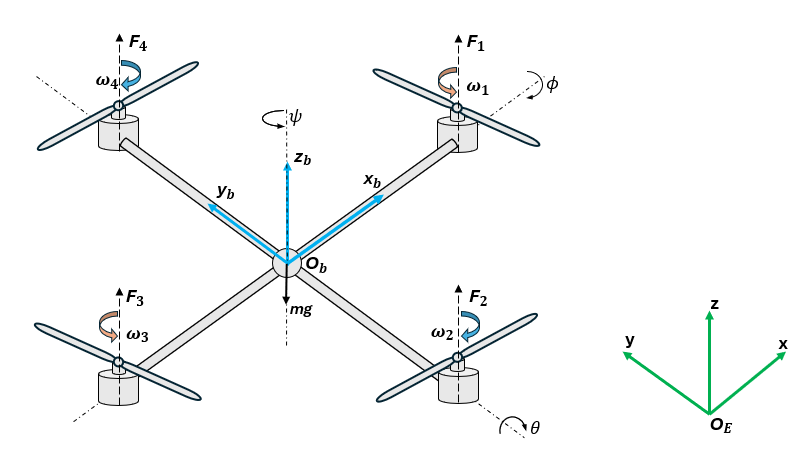
\includegraphics[width=0.92\textwidth]{model.png}
\caption{Mô hình của Quadcopter với hệ tọa độ quán tính $E$ và hệ tọa độ thân $B$.}
\label{fig:pos_tracking}
\end{figure}

Để mô tả chuyển động của Quadcopter trong không gian ba chiều, cần định nghĩa hai hệ tọa độ.

Hệ tọa độ quán tính $E = \{O_E, X_E, Y_E, Z_E\}$ là hệ tọa độ cố định gắn với mặt đất. Trục $Z_E$ hướng lên trên theo chiều ngược với trọng lực. Hệ này được dùng làm hệ quy chiếu để xác định vị trí và hướng của Quadcopter.

Hệ tọa độ thân $B = \{O_B, X_B, Y_B, Z_B\}$ có gốc đặt tại trọng tâm của Quadcopter và quay cùng với thân máy bay. Trục $X_B$ hướng về phía trước, trục $Y_B$ hướng sang trái, trục $Z_B$ hướng lên trên theo quy tắc bàn tay phải.

Vị trí trọng tâm của Quadcopter trong hệ $E$ được xác định bởi vec-tơ:
\begin{equation}
\xi = \begin{bmatrix} x \\ y \\ z \end{bmatrix}
\end{equation}

Tư thế của Quadcopter được mô tả bằng ba góc Euler: góc roll $\phi$ quay quanh trục $X_B$, góc pitch $\theta$ quay quanh trục $Y_B$, và góc yaw $\psi$ quay quanh trục $Z_B$:
\begin{equation}
\eta = \begin{bmatrix} \phi \\ \theta \\ \psi \end{bmatrix}
\end{equation}

\section{Ma trận quay}
Ma trận quay $R$ biến đổi một vec-tơ từ hệ tọa độ thân $B$ sang hệ tọa độ quán tính $E$. Ma trận này được xây dựng bằng cách nhân lần lượt ba ma trận quay cơ bản theo thứ tự Z-Y-X.

Ma trận quay quanh trục $Z$ một góc $\psi$:
\begin{equation}
R_z(\psi) = \begin{bmatrix}
\cos\psi & -\sin\psi & 0 \\
\sin\psi & \cos\psi  & 0 \\
0        & 0         & 1
\end{bmatrix}
\end{equation}

Ma trận quay quanh trục $Y$ một góc $\theta$:
\begin{equation}
R_y(\theta) = \begin{bmatrix}
\cos\theta  & 0 & \sin\theta \\
0           & 1 & 0          \\
-\sin\theta & 0 & \cos\theta
\end{bmatrix}
\end{equation}

Ma trận quay quanh trục $X$ một góc $\phi$:
\begin{equation}
R_x(\phi) = \begin{bmatrix}
1 & 0        & 0         \\
0 & \cos\phi & -\sin\phi \\
0 & \sin\phi & \cos\phi
\end{bmatrix}
\end{equation}

Tích ba ma trận theo thứ tự $R = R_z(\psi) \cdot R_y(\theta) \cdot R_x(\phi)$ cho kết quả:
\begin{equation}
R = \begin{bmatrix}
c\theta c\psi & s\phi s\theta c\psi - c\phi s\psi & c\phi s\theta c\psi + s\phi s\psi \\[6pt]
c\theta s\psi & s\phi s\theta s\psi + c\phi c\psi & c\phi s\theta s\psi - s\phi c\psi \\[6pt]
-s\theta      & s\phi c\theta                     & c\phi c\theta
\end{bmatrix}
\end{equation}
trong đó ký hiệu $c$ và $s$ lần lượt thay cho $\cos$ và $\sin$. Ma trận $R$ là ma trận trực giao, thỏa mãn $R^T R = I$ và $\det(R) = 1$.

\section{Mô hình lực và moment từ cánh quạt}
Mỗi cánh quạt quay với vận tốc góc $\omega_i$ sinh ra một lực đẩy hướng lên theo trục $Z_B$ và một moment phản lực quanh trục quay. Các đại lượng này được tính theo:
\begin{equation}
F_i = k_F \omega_i^2, \quad M_i = k_M \omega_i^2
\end{equation}
trong đó $k_F$ là hệ số lực đẩy và $k_M$ là hệ số moment, cả hai phụ thuộc vào hình dạng cánh quạt và mật độ không khí.

Bốn cánh quạt được bố trí đối xứng hình chữ thập, đánh số từ 1 đến 4 theo thứ tự trước, phải, sau, trái. Cánh quạt 1 và 3 quay cùng chiều, cánh quạt 2 và 4 quay ngược lại để triệt tiêu moment phản lực tổng khi hovering.

Lực nâng tổng $U_1$, moment roll $U_2$, moment pitch $U_3$ và moment yaw $U_4$ được xác định từ lực đẩy của từng cánh quạt:
\begin{equation}
\begin{bmatrix} U_1 \\[4pt] U_2 \\[4pt] U_3 \\[4pt] U_4 \end{bmatrix}
=
\begin{bmatrix}
1    & 1     & 1    & 1     \\[4pt]
0    & -l    & 0    & l     \\[4pt]
l    & 0     & -l   & 0     \\[4pt]
-\kappa & \kappa & -\kappa & \kappa
\end{bmatrix}
\begin{bmatrix} F_1 \\[4pt] F_2 \\[4pt] F_3 \\[4pt] F_4 \end{bmatrix}
\end{equation}
trong đó $\kappa = k_M / k_F$ là tỉ số moment trên lực và $l$ là chiều dài cánh tay đòn. Ma trận $4 \times 4$ ở trên gọi là ma trận phân bổ, cho phép chuyển đổi qua lại giữa tín hiệu điều khiển tổng hợp $U_1, U_2, U_3, U_4$ và lực đẩy riêng lẻ $F_1, F_2, F_3, F_4$.

Tổng vận tốc góc dư của các rotor, gây ra hiệu ứng con quay hồi chuyển, được định nghĩa:
\begin{equation}
\omega_r = -\omega_1 + \omega_2 - \omega_3 + \omega_4
\end{equation}
Dấu luân phiên phản ánh chiều quay ngược nhau giữa các cánh quạt liền kề.

\section{Động lực học tịnh tiến}
Áp dụng định luật II Newton cho chuyển động tịnh tiến của trọng tâm Quadcopter trong hệ tọa độ quán tính $E$~\cite{bouabdallah2004,khalil2002}:
\begin{equation}
m \ddot{\xi} = F_g + F_T + F_d
\end{equation}
trong đó $m$ là khối lượng, $F_g$ là lực trọng trường, $F_T$ là lực đẩy tổng, $F_d$ là lực cản khí động học.

Lực trọng trường tác dụng theo phương $Z_E$ hướng xuống:
\begin{equation}
F_g = \begin{bmatrix} 0 \\ 0 \\ -mg \end{bmatrix}
\end{equation}

Lực đẩy tổng $U_1$ hướng theo trục $Z_B$ của hệ tọa độ thân. Để biểu diễn trong hệ $E$, cần nhân với ma trận quay $R$:
\begin{equation}
F_T = R \begin{bmatrix} 0 \\ 0 \\ U_1 \end{bmatrix}
= U_1 \begin{bmatrix} c\phi s\theta c\psi + s\phi s\psi \\[6pt] c\phi s\theta s\psi - s\phi c\psi \\[6pt] c\phi c\theta \end{bmatrix}
\end{equation}
Vec-tơ kết quả cho thấy lực đẩy $U_1$ được phân bổ lên cả ba trục $x$, $y$, $z$ tùy thuộc vào tư thế hiện tại của Quadcopter. Khi Quadcopter nằm ngang hoàn toàn ($\phi = \theta = 0$), toàn bộ lực đẩy hướng lên theo trục $z$.

Lực cản khí động học được mô hình hóa tuyến tính theo vận tốc:
\begin{equation}
F_d = -\begin{bmatrix} k_{dx} \dot{x} \\[6pt] k_{dy} \dot{y} \\[6pt] k_{dz} \dot{z} \end{bmatrix}
\end{equation}

Thay các thành phần vào phương trình Newton và chia cho $m$, ta được hệ phương trình tịnh tiến:
\begin{equation}
\begin{cases}
\ddot{x} = \dfrac{U_1}{m} (c\phi \, s\theta \, c\psi + s\phi \, s\psi) - \dfrac{k_{dx}}{m} \dot{x} \\[10pt]
\ddot{y} = \dfrac{U_1}{m} (c\phi \, s\theta \, s\psi - s\phi \, c\psi) - \dfrac{k_{dy}}{m} \dot{y} \\[10pt]
\ddot{z} = \dfrac{U_1}{m} c\phi \, c\theta - g - \dfrac{k_{dz}}{m} \dot{z}
\end{cases}
\end{equation}

Phương trình trục $z$ cho thấy để Quadcopter hovering ổn định ($\ddot{z} = 0$, $\dot{z} = 0$, $\phi = \theta = 0$), lực nâng cần bằng đúng trọng lực: $U_1 = mg$. Với các thông số trong bảng 1.1, giá trị này là $U_1 = 1.10 \times 9.81 = 10.791$ N.

\section{Động lực học quay}
Phương trình Euler cho chuyển động quay của vật rắn quanh trọng tâm trong hệ tọa độ thân:
\begin{equation}
I \dot{\Omega}_B + \Omega_B \times (I \Omega_B) = \tau
\end{equation}
trong đó $I$ là ma trận moment quán tính, $\Omega_B = [\dot{\phi}, \dot{\theta}, \dot{\psi}]^T$ là vec-tơ vận tốc góc trong hệ thân, $\tau$ là vec-tơ moment ngoại lực.

Do cấu hình đối xứng của Quadcopter, ma trận moment quán tính là ma trận đường chéo:
\begin{equation}
I = \begin{bmatrix} I_x & 0 & 0 \\ 0 & I_y & 0 \\ 0 & 0 & I_z \end{bmatrix}
\end{equation}

Thực hiện phép nhân vec-tơ chéo $\Omega_B \times (I \Omega_B)$:
\begin{equation}
\Omega_B \times (I \Omega_B) = \begin{bmatrix} \dot{\phi} \\ \dot{\theta} \\ \dot{\psi} \end{bmatrix} \times \begin{bmatrix} I_x \dot{\phi} \\ I_y \dot{\theta} \\ I_z \dot{\psi} \end{bmatrix} = \begin{bmatrix} (I_z - I_y) \dot{\theta} \dot{\psi} \\ (I_x - I_z) \dot{\phi} \dot{\psi} \\ (I_y - I_x) \dot{\phi} \dot{\theta} \end{bmatrix}
\end{equation}

Ngoài moment từ chênh lệch lực đẩy giữa các cánh quạt, sự quay của các rotor còn tạo ra hiệu ứng con quay hồi chuyển. Khi thân Quadcopter quay với vận tốc góc $\Omega_B$ trong khi các rotor đang quay với tổng vận tốc dư $\omega_r$, moment hồi chuyển sinh ra là:
\begin{equation}
\tau_{gyro} = I_r \begin{bmatrix} -\dot{\theta} \, \omega_r \\[6pt] \dot{\phi} \, \omega_r \\[6pt] 0 \end{bmatrix}
\end{equation}
trong đó $I_r$ là moment quán tính của mỗi rotor quanh trục quay. Thành phần moment hồi chuyển theo trục yaw bằng không vì $\omega_r$ quay cùng phương với trục $Z_B$.

Vec-tơ moment ngoại lực tổng gồm moment từ các cánh quạt và moment hồi chuyển:
\begin{equation}
\tau = \begin{bmatrix} l \, U_2 \\[6pt] l \, U_3 \\[6pt] U_4 \end{bmatrix} - \tau_{gyro}
\end{equation}

Thay vào phương trình Euler và khai triển từng thành phần:
\begin{equation}
\begin{cases}
I_x \ddot{\phi} = (I_y - I_z) \dot{\theta} \dot{\psi} - I_r \dot{\theta} \, \omega_r + l \, U_2 \\[10pt]
I_y \ddot{\theta} = (I_z - I_x) \dot{\phi} \dot{\psi} + I_r \dot{\phi} \, \omega_r + l \, U_3 \\[10pt]
I_z \ddot{\psi} = (I_x - I_y) \dot{\phi} \dot{\theta} + U_4
\end{cases}
\end{equation}

Chia mỗi phương trình cho moment quán tính tương ứng:
\begin{equation}
\begin{cases}
\ddot{\phi} = \dfrac{I_y - I_z}{I_x} \dot{\theta} \dot{\psi} - \dfrac{I_r}{I_x} \dot{\theta} \, \omega_r + \dfrac{l}{I_x} U_2 \\[10pt]
\ddot{\theta} = \dfrac{I_z - I_x}{I_y} \dot{\phi} \dot{\psi} + \dfrac{I_r}{I_y} \dot{\phi} \, \omega_r + \dfrac{l}{I_y} U_3 \\[10pt]
\ddot{\psi} = \dfrac{I_x - I_y}{I_z} \dot{\phi} \dot{\theta} + \dfrac{1}{I_z} U_4
\end{cases}
\end{equation}

Mỗi phương trình có dạng $\ddot{q} = f_q + b_q \, U_q$, trong đó $f_q$ gộp các thành phần phi tuyến ghép nối và $b_q$ là hệ số điều khiển. Cụ thể, với trục roll:
\begin{equation}
f_\phi = \frac{I_y - I_z}{I_x} \dot{\theta} \dot{\psi} - \frac{I_r}{I_x} \dot{\theta} \, \omega_r, \quad b_\phi = \frac{l}{I_x}
\end{equation}

Tương tự cho trục pitch và yaw:
\begin{equation}
f_\theta = \frac{I_z - I_x}{I_y} \dot{\phi} \dot{\psi} + \frac{I_r}{I_y} \dot{\phi} \, \omega_r, \quad b_\theta = \frac{l}{I_y}
\end{equation}
\begin{equation}
f_\psi = \frac{I_x - I_y}{I_z} \dot{\phi} \dot{\theta}, \quad b_\psi = \frac{1}{I_z}
\end{equation}

\section{Dạng rút gọn cho thiết kế điều khiển}
Để thuận tiện cho việc thiết kế bộ điều khiển ở các chương sau, các phương trình tịnh tiến cũng được viết lại dưới dạng tương tự. Đặt các tín hiệu điều khiển ảo:
\begin{equation}
u_x = c\phi \, s\theta \, c\psi + s\phi \, s\psi, \quad u_y = c\phi \, s\theta \, s\psi - s\phi \, c\psi
\end{equation}

Phương trình tịnh tiến trở thành:
\begin{equation}
\begin{cases}
\ddot{x} = \dfrac{U_1}{m} u_x - \dfrac{k_{dx}}{m} \dot{x} \\[10pt]
\ddot{y} = \dfrac{U_1}{m} u_y - \dfrac{k_{dy}}{m} \dot{y} \\[10pt]
\ddot{z} = \dfrac{U_1}{m} c\phi \, c\theta - g - \dfrac{k_{dz}}{m} \dot{z}
\end{cases}
\end{equation}

Tín hiệu $u_x$ và $u_y$ phụ thuộc vào các góc $\phi$, $\theta$, $\psi$. Khi biết các giá trị mong muốn $u_x$ và $u_y$ từ bộ điều khiển vị trí, có thể suy ngược ra góc tham chiếu $\phi_d$ và $\theta_d$ thông qua phép biến đổi lượng giác ngược. Với góc yaw mong muốn $\psi_d$ đã cho trước:
\begin{equation}
\phi_d = \arcsin(u_x \sin\psi_d - u_y \cos\psi_d)
\end{equation}
\begin{equation}
\theta_d = \arcsin\left(\frac{u_x \cos\psi_d + u_y \sin\psi_d}{\cos\phi_d}\right)
\end{equation}

Các công thức nghịch đảo này là cầu nối giữa vòng điều khiển ngoài và vòng điều khiển trong của cấu trúc tầng. Giá trị $u_x$ và $u_y$ cần được giới hạn trong khoảng $[-1, 1]$ để đảm bảo hàm $\arcsin$ có nghiệm, tương ứng với việc giới hạn góc nghiêng thân Quadcopter trong phạm vi cho phép.

Tổng hợp lại, mô hình toán học đầy đủ của Quadcopter gồm 12 biến trạng thái: 6 biến vị trí và góc $(x, y, z, \phi, \theta, \psi)$ cùng 6 biến vận tốc tương ứng $(\dot{x}, \dot{y}, \dot{z}, \dot{\phi}, \dot{\theta}, \dot{\psi})$, được điều khiển bởi 4 tín hiệu đầu vào $U_1, U_2, U_3, U_4$.

% --- CHƯƠNG 3 ---
\chapter{THIẾT KẾ BỘ ĐIỀU KHIỂN}

Chương này trình bày chi tiết việc áp dụng thuật toán Super-Twisting SMC cho từng kênh điều khiển của Quadcopter theo cấu trúc tầng đã giới thiệu ở Chương 1. Quá trình thiết kế được thực hiện lần lượt cho vòng ngoài rồi đến vòng trong.
\section{Sơ đồ khối bộ điều khiển}

\begin{figure}[h!]
\centering
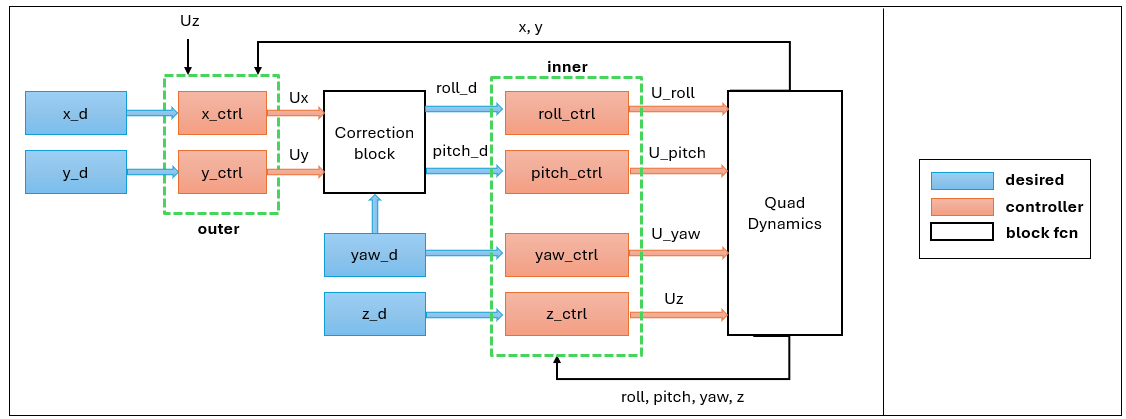
\includegraphics[width=0.92\textwidth]{bdk.png}
\caption{Sơ đồ khối bộ điều khiển}
\label{fig:controller_block_diagram}
\end{figure}

\section{Thiết kế chung cho một kênh}
Xét một kênh điều khiển tổng quát có phương trình động lực học dạng~\cite{shtessel2014}:
\begin{equation}
\ddot{q} = f(q, \dot{q}, t) + b \cdot u + w(t)
\end{equation}
trong đó $q$ là biến trạng thái, $u$ là tín hiệu điều khiển, $f$ là thành phần phi tuyến đã biết, $b$ là hệ số điều khiển, $w(t)$ là nhiễu bất định thỏa mãn $|w(t)| \le W$.

Đặt sai số bám $e = q_d - q$ với $q_d$ là tín hiệu đặt. Mặt trượt được chọn:
\begin{equation}
s = \dot{e} + \lambda e
\end{equation}
với $\lambda > 0$.

Đạo hàm mặt trượt theo thời gian:
\begin{equation}
\dot{s} = \ddot{e} + \lambda \dot{e} = (\ddot{q}_d - \ddot{q}) + \lambda \dot{e}
\end{equation}

Thay phương trình động lực học vào:
\begin{equation}
\dot{s} = \ddot{q}_d - f - b \cdot u - w + \lambda \dot{e}
\end{equation}

Luật điều khiển được thiết kế gồm hai thành phần $u = u_{eq} + u_{st}$.

Thành phần tương đương $u_{eq}$ bù các phần đã biết, đặt $\dot{s} = 0$ khi $w = 0$:
\begin{equation}
u_{eq} = \frac{1}{b} (\ddot{q}_d - f + \lambda \dot{e})
\end{equation}

Thành phần Super-Twisting $u_{st}$ xử lý nhiễu và đảm bảo hội tụ:
\begin{equation}
u_{st} = \frac{1}{b} \left( c_1 |s|^{1/2} \text{sgn}(s) + v \right)
\end{equation}
\begin{equation}
\dot{v} = c_2 \, \text{sgn}(s)
\end{equation}
trong đó $v$ là biến tích phân nội bộ, $c_1 > 0$ và $c_2 > 0$ là hai hệ số thiết kế.

Luật điều khiển tổng hợp:
\begin{equation}
u = \frac{1}{b} \left( \ddot{q}_d - f + \lambda \dot{e} + c_1 |s|^{1/2} \text{sgn}(s) + v \right)
\end{equation}

Thay luật điều khiển vào phương trình $\dot{s}$, phần đã biết bị triệt tiêu hoàn toàn, còn lại:
\begin{equation}
\dot{s} = -c_1 |s|^{1/2} \text{sgn}(s) - v + w(t)
\end{equation}

Đây chính là dạng chuẩn của thuật toán Super-Twisting, sẽ được phân tích ổn định ở Chương 4.

\section{Vòng ngoài: điều khiển độ cao $z$}
Từ phương trình tịnh tiến trục $z$ ở Chương 2:
\begin{equation}
\ddot{z} = \frac{U_1}{m} \cos\phi \cos\theta - g - \frac{k_{dz}}{m} \dot{z}
\end{equation}

Đặt sai số $e_z = z_d - z$ và mặt trượt $s_z = \dot{e}_z + \lambda_z e_z$. Đạo hàm mặt trượt:
\begin{equation}
\dot{s}_z = \ddot{z}_d - \ddot{z} + \lambda_z \dot{e}_z
= \ddot{z}_d - \frac{U_1}{m} \cos\phi \cos\theta + g + \frac{k_{dz}}{m} \dot{z} + \lambda_z \dot{e}_z
\end{equation}

Đặt $\dot{s}_z = -c_{1,z} |s_z|^{1/2} \text{sgn}(s_z) - v_z$ và giải ra $U_1$:
\begin{equation}
U_1 = \frac{m}{\cos\phi \cos\theta} \left( \ddot{z}_d + g + \frac{k_{dz}}{m} \dot{z} + \lambda_z \dot{e}_z + c_{1,z} |s_z|^{1/2} \text{sgn}(s_z) + v_z \right)
\end{equation}
\begin{equation}
\dot{v}_z = c_{2,z} \, \text{sgn}(s_z)
\end{equation}

Giá trị $U_1$ cần được giới hạn trong khoảng $[U_{z,\min}, \, U_{z,\max}]$ với $U_{z,\min} = 0$ và $U_{z,\max} = 3.2 \, mg$ để đảm bảo lực đẩy không vượt quá khả năng của động cơ. Hệ số $\cos\phi \cos\theta$ ở mẫu số đòi hỏi các góc $\phi$ và $\theta$ phải nằm trong khoảng $(-90^\circ, 90^\circ)$, điều này luôn thỏa mãn trong chế độ bay bình thường.

\section{Vòng ngoài: điều khiển vị trí $x$ và $y$}
Phương trình tịnh tiến trục $x$:
\begin{equation}
\ddot{x} = \frac{U_1}{m} u_x - \frac{k_{dx}}{m} \dot{x}
\end{equation}
với $u_x = \cos\phi \sin\theta \cos\psi + \sin\phi \sin\psi$.

Đặt sai số $e_x = x_d - x$ và mặt trượt $s_x = \dot{e}_x + \lambda_x e_x$. Áp dụng luật STSMC, ta tính tín hiệu ảo $u_x$:
\begin{equation}
u_x = \frac{m}{U_1} \left( \ddot{x}_d + \frac{k_{dx}}{m} \dot{x} + \lambda_x \dot{e}_x + c_{1,x} |s_x|^{1/2} \text{sgn}(s_x) + v_x \right)
\end{equation}
\begin{equation}
\dot{v}_x = c_{2,x} \, \text{sgn}(s_x)
\end{equation}

Tương tự cho trục $y$:
\begin{equation}
u_y = \frac{m}{U_1} \left( \ddot{y}_d + \frac{k_{dy}}{m} \dot{y} + \lambda_y \dot{e}_y + c_{1,y} |s_y|^{1/2} \text{sgn}(s_y) + v_y \right)
\end{equation}
\begin{equation}
\dot{v}_y = c_{2,y} \, \text{sgn}(s_y)
\end{equation}

Giá trị $u_x$ và $u_y$ được giới hạn trong khoảng $[-U_{xy,\max}, \, U_{xy,\max}]$ với $U_{xy,\max} = 0.2$ để Quadcopter không nghiêng quá mức.

\subsection{Tính góc tham chiếu}
Từ các tín hiệu ảo $u_x$ và $u_y$, góc tham chiếu cho vòng trong được suy ra bằng phép nghịch đảo đã trình bày ở Chương 2:
\begin{equation}
\phi_d = \arcsin(u_x \sin\psi_d - u_y \cos\psi_d)
\end{equation}
\begin{equation}
\theta_d = \arcsin\left(\frac{u_x \cos\psi_d + u_y \sin\psi_d}{\cos\phi_d}\right)
\end{equation}

Các góc $\phi_d$ và $\theta_d$ được giới hạn thêm bởi $\phi_{d,\max} = \theta_{d,\max} = 6^\circ$ để giữ Quadcopter hoạt động trong vùng góc nhỏ, nơi các xấp xỉ tuyến tính của mô hình vẫn có giá trị.

\subsection{Bộ lọc cho góc tham chiếu}
Các góc $\phi_d$ và $\theta_d$ sinh ra từ vòng ngoài có thể thay đổi nhanh khi sai số vị trí lớn. Nếu đưa trực tiếp vào vòng trong, tín hiệu đặt sẽ không mượt và có thể gây ra dao động. Để xử lý vấn đề này, các góc tham chiếu được cho qua bộ lọc bậc hai có dạng:
\begin{equation}
H(s) = \frac{\omega_n^2}{s^2 + 2\zeta\omega_n s + \omega_n^2}
\end{equation}
với $\omega_n = 3.0$ rad/s là tần số tự nhiên và $\zeta = 1.1$ là hệ số tắt dần. Giá trị $\zeta > 1$ đảm bảo bộ lọc ở chế độ quá tắt dần, không gây vọt lố trên tín hiệu góc tham chiếu.

Bộ lọc này đồng thời cung cấp các đạo hàm $\dot{\phi}_d$, $\ddot{\phi}_d$, $\dot{\theta}_d$, $\ddot{\theta}_d$ cần thiết cho luật điều khiển vòng trong mà không cần tính đạo hàm số gây nhiễu.

\section{Vòng trong: điều khiển góc roll $\phi$}
Từ phương trình quay trục roll ở Chương 2:
\begin{equation}
\ddot{\phi} = f_\phi + b_\phi U_2
\end{equation}
với $f_\phi = \dfrac{I_y - I_z}{I_x} \dot{\theta} \dot{\psi} - \dfrac{I_r}{I_x} \dot{\theta} \, \omega_r$ và $b_\phi = \dfrac{l}{I_x}$.

Đặt sai số $e_\phi = \phi_d - \phi$ và mặt trượt $s_\phi = \dot{e}_\phi + \lambda_\phi e_\phi$. Luật điều khiển STSMC cho moment roll:
\begin{equation}
U_2 = \frac{1}{b_\phi} \left( \ddot{\phi}_d - f_\phi + \lambda_\phi \dot{e}_\phi + c_{1,\phi} |s_\phi|^{1/2} \text{sgn}(s_\phi) + v_\phi \right)
\end{equation}
\begin{equation}
\dot{v}_\phi = c_{2,\phi} \, \text{sgn}(s_\phi)
\end{equation}

Thay $b_\phi = l / I_x$:
\begin{equation}
U_2 = \frac{I_x}{l} \left( \ddot{\phi}_d - f_\phi + \lambda_\phi \dot{e}_\phi + c_{1,\phi} |s_\phi|^{1/2} \text{sgn}(s_\phi) + v_\phi \right)
\end{equation}

Giá trị $U_2$ được giới hạn trong khoảng $[-M_{\phi,\max}, \, M_{\phi,\max}]$ với $M_{\phi,\max} = 0.22$ Nm.

\section{Vòng trong: điều khiển góc pitch $\theta$}
Do cấu hình đối xứng $I_x = I_y$, luật điều khiển trục pitch có cùng cấu trúc với trục roll:
\begin{equation}
U_3 = \frac{I_y}{l} \left( \ddot{\theta}_d - f_\theta + \lambda_\theta \dot{e}_\theta + c_{1,\theta} |s_\theta|^{1/2} \text{sgn}(s_\theta) + v_\theta \right)
\end{equation}
\begin{equation}
\dot{v}_\theta = c_{2,\theta} \, \text{sgn}(s_\theta)
\end{equation}
với $f_\theta = \dfrac{I_z - I_x}{I_y} \dot{\phi} \dot{\psi} + \dfrac{I_r}{I_y} \dot{\phi} \, \omega_r$. Giới hạn $|U_3| \le M_{\theta,\max} = 0.22$ Nm.

\section{Vòng trong: điều khiển góc yaw $\psi$}
Phương trình trục yaw:
\begin{equation}
\ddot{\psi} = f_\psi + b_\psi U_4
\end{equation}
với $f_\psi = \dfrac{I_x - I_y}{I_z} \dot{\phi} \dot{\theta}$ và $b_\psi = \dfrac{1}{I_z}$.

Luật điều khiển:
\begin{equation}
U_4 = I_z \left( \ddot{\psi}_d - f_\psi + \lambda_\psi \dot{e}_\psi + c_{1,\psi} |s_\psi|^{1/2} \text{sgn}(s_\psi) + v_\psi \right)
\end{equation}
\begin{equation}
\dot{v}_\psi = c_{2,\psi} \, \text{sgn}(s_\psi)
\end{equation}
Giới hạn $|U_4| \le M_{\psi,\max} = 0.08$ Nm. Giá trị này nhỏ hơn so với roll và pitch vì moment quán tính $I_z = 0.040$ lớn hơn nhưng trục yaw thường không cần đáp ứng nhanh.

\section{Bảng tham số bộ điều khiển}
Toàn bộ tham số của bộ điều khiển STSMC được tổng hợp trong Bảng~\ref{tab:ctrl_params}.

\begin{table}[h!]
\centering
\caption{Tham số bộ điều khiển STSMC}
\label{tab:ctrl_params}
\renewcommand{\arraystretch}{1.3}
\begin{tabular}{|l|c|c|c|c|c|c|}
\hline
Tham số & $x$ & $y$ & $z$ & $\phi$ & $\theta$ & $\psi$ \\
\hline
$\lambda$ & 0.55 & 0.55 & 2.3 & 6.0 & 6.0 & 3.0 \\
$c_1$ & 0.08 & 0.08 & 1.9 & 1.60 & 1.60 & 0.18 \\
$c_2$ & 0.015 & 0.015 & 1.8 & 0.70 & 0.70 & 0.25 \\
Giới hạn tín hiệu & 0.2 & 0.2 & $3.2mg$ & 0.22 & 0.22 & 0.08 \\
\hline
\end{tabular}
\end{table}

Một số nhận xét về việc chọn tham số:

Hệ số $\lambda$ của vòng trong ($\lambda_\phi = \lambda_\theta = 6.0$) lớn hơn nhiều so với vòng ngoài ($\lambda_x = \lambda_y = 0.55$). Điều này phản ánh yêu cầu vòng trong phải có tốc độ đáp ứng nhanh hơn để kịp bám theo góc tham chiếu do vòng ngoài sinh ra.

Hệ số $c_1$ và $c_2$ của kênh $z$ ($c_{1,z} = 1.9$, $c_{2,z} = 1.8$) lớn hơn đáng kể so với kênh $x$, $y$ ($c_{1,x} = 0.08$, $c_{2,x} = 0.015$). Lý do là kênh $z$ phải bù trực tiếp trọng lực và chịu nhiễu cản khí động học lớn hơn, trong khi kênh $x$, $y$ điều khiển gián tiếp qua góc nghiêng nên tín hiệu ảo $u_x$, $u_y$ có biên độ nhỏ.

Giới hạn góc tham chiếu $\phi_{d,\max} = \theta_{d,\max} = 6^\circ$ giữ cho Quadcopter hoạt động trong vùng góc nhỏ. Trong vùng này, $\sin\phi \approx \phi$ và $\cos\phi \approx 1$, giúp mối liên hệ giữa lực tịnh tiến và góc nghiêng gần như tuyến tính.

Các tham số bổ sung khác gồm tham số lớp ranh giới $\phi_{bl} = 0.12$, tham số căn $\epsilon = 5 \times 10^{-5}$, và bước tính $T_s = 0.001$ s. Thời gian mô phỏng mặc định là $100$ s.


% --- CHƯƠNG 4 ---
\chapter{CHỨNG MINH ỔN ĐỊNH}

Chương này chứng minh rằng thuật toán Super-Twisting đảm bảo mặt trượt $s$ hội tụ về $0$ trong thời gian hữu hạn, từ đó sai số bám $e$ cũng tiến về $0$. Phương pháp chứng minh sử dụng hàm Lyapunov theo cách tiếp cận của Moreno và Osorio~\cite{moreno2012}.

\section{Hệ động lực vòng kín}
Từ kết quả ở Chương 3, sau khi thay luật điều khiển STSMC vào phương trình $\dot{s}$, thành phần tương đương $u_{eq}$ triệt tiêu các phần đã biết. Phần còn lại có dạng:
\begin{equation}
\dot{s} = -c_1 |s|^{1/2} \text{sgn}(s) + v + w(t)
\end{equation}
\begin{equation}
\dot{v} = -c_2 \, \text{sgn}(s)
\end{equation}
trong đó $v$ là biến tích phân nội bộ của thuật toán Super-Twisting và $w(t)$ đại diện cho nhiễu bất định gộp, bao gồm sai số mô hình và nhiễu ngoại sinh.

Giả thiết nhiễu thỏa mãn: $w(t)$ bị chặn và có đạo hàm bị chặn, tức là tồn tại hằng số $L > 0$ sao cho $|\dot{w}(t)| \le L$ với mọi $t \ge 0$. Giả thiết này phù hợp với thực tế vì nhiễu vật lý luôn có tốc độ biến thiên hữu hạn.

\section{Đổi biến trạng thái}
Hệ phương trình trên có tính kỳ dị tại $s = 0$ do thành phần $|s|^{1/2}$. Để phân tích ổn định, ta thực hiện phép đổi biến:
\begin{equation}
z_1 = |s|^{1/2} \text{sgn}(s), \quad z_2 = v + w(t)
\end{equation}

Từ định nghĩa $z_1$, ta có $s = z_1 |z_1|$ và $|s|^{1/2} = |z_1|$. Đạo hàm $z_1$ theo thời gian:
\begin{equation}
\dot{z}_1 = \frac{\dot{s}}{2|s|^{1/2}} = \frac{\dot{s}}{2|z_1|}
\end{equation}

Thay biểu thức $\dot{s}$ vào:
\begin{equation}
\dot{z}_1 = \frac{1}{2|z_1|} \left( -c_1 |z_1| \, \text{sgn}(z_1) + z_2 \right)
\end{equation}

Vì $|z_1| \, \text{sgn}(z_1) = z_1$, ta được:
\begin{equation}
\dot{z}_1 = \frac{1}{2|z_1|} (-c_1 z_1 + z_2)
\end{equation}

Đạo hàm $z_2$:
\begin{equation}
\dot{z}_2 = \dot{v} + \dot{w} = -c_2 \, \text{sgn}(s) + \dot{w}
\end{equation}

Vì $\text{sgn}(s) = \text{sgn}(z_1)$ và $\text{sgn}(z_1) = z_1 / |z_1|$:
\begin{equation}
\dot{z}_2 = -c_2 \frac{z_1}{|z_1|} + \dot{w}
\end{equation}

Nhân và chia cho $2|z_1|$ ở vế phải:
\begin{equation}
\dot{z}_2 = \frac{1}{2|z_1|} (-2c_2 z_1 + 2|z_1| \dot{w})
\end{equation}

Viết hệ phương trình dưới dạng ma trận:
\begin{equation}
\dot{z} = \frac{1}{2|z_1|} \left( A z + B \dot{w} \right)
\end{equation}
với:
\begin{equation}
z = \begin{bmatrix} z_1 \\ z_2 \end{bmatrix}, \quad
A = \begin{bmatrix} -c_1 & 1 \\ -2c_2 & 0 \end{bmatrix}, \quad
B = \begin{bmatrix} 0 \\ 2|z_1| \end{bmatrix}
\end{equation}

Ma trận $A$ có đa thức đặc trưng $\det(\lambda I - A) = \lambda^2 + c_1 \lambda + 2c_2$. Với $c_1 > 0$ và $c_2 > 0$, theo tiêu chuẩn Hurwitz, cả hai nghiệm đều có phần thực âm, nên $A$ là ma trận Hurwitz.

\section{Xây dựng hàm Lyapunov}
Chọn hàm Lyapunov dạng toàn phương:
\begin{equation}
V(z) = z^T P z
\end{equation}
với $P$ là ma trận đối xứng xác định dương cần xác định.

Chọn $P$ theo dạng:
\begin{equation}
P = \frac{1}{2} \begin{bmatrix} 4c_2 + c_1^2 & -c_1 \\ -c_1 & 2 \end{bmatrix}
\end{equation}

Kiểm tra $P$ xác định dương. Các giá trị riêng của $P$ dương khi và chỉ khi:
\begin{itemize}
\item $P_{11} = \frac{4c_2 + c_1^2}{2} > 0$: luôn đúng với $c_1, c_2 > 0$.
\item $\det(P) = \frac{1}{4}(2(4c_2 + c_1^2) - c_1^2) = \frac{1}{4}(8c_2 + c_1^2) > 0$: luôn đúng.
\end{itemize}
Vậy $P$ xác định dương.

Khai triển $V(z)$:
\begin{equation}
V(z) = \frac{1}{2}(4c_2 + c_1^2) z_1^2 - c_1 z_1 z_2 + z_2^2
\end{equation}

Vì $P$ xác định dương, tồn tại các hằng số $\lambda_{\min}(P) > 0$ và $\lambda_{\max}(P) > 0$ sao cho:
\begin{equation}
\lambda_{\min}(P) \|z\|^2 \le V(z) \le \lambda_{\max}(P) \|z\|^2
\end{equation}

\section{Tính đạo hàm hàm Lyapunov}
Đạo hàm $V$ theo thời gian:
\begin{equation}
\dot{V} = \dot{z}^T P z + z^T P \dot{z} = 2 z^T P \dot{z}
\end{equation}

Thay $\dot{z}$:
\begin{equation}
\dot{V} = \frac{2}{2|z_1|} z^T P (Az + B\dot{w}) = \frac{1}{|z_1|} \left( z^T P A z + z^T P B \dot{w} \right)
\end{equation}

Vì $z^T P A z = \frac{1}{2} z^T (PA + A^T P) z$:
\begin{equation}
\dot{V} = \frac{1}{|z_1|} \left( \frac{1}{2} z^T (PA + A^T P) z + z^T P B \dot{w} \right)
\end{equation}

Tính tích $PA + A^T P$. Đặt $Q_0 = -(PA + A^T P)$:
\begin{equation}
PA = \frac{1}{2} \begin{bmatrix} 4c_2 + c_1^2 & -c_1 \\ -c_1 & 2 \end{bmatrix} \begin{bmatrix} -c_1 & 1 \\ -2c_2 & 0 \end{bmatrix}
\end{equation}
\begin{equation}
= \frac{1}{2} \begin{bmatrix} -c_1(4c_2 + c_1^2) + 2c_1 c_2 & 4c_2 + c_1^2 \\ c_1^2 - 4c_2 & -c_1 \end{bmatrix}
\end{equation}
\begin{equation}
= \frac{1}{2} \begin{bmatrix} -c_1^3 - 2c_1 c_2 & 4c_2 + c_1^2 \\ c_1^2 - 4c_2 & -c_1 \end{bmatrix}
\end{equation}

Cộng với chuyển vị $(PA)^T = A^T P$:
\begin{equation}
PA + A^T P = \frac{1}{2} \begin{bmatrix} -2c_1^3 - 4c_1 c_2 & 2c_1^2 \\ 2c_1^2 & -2c_1 \end{bmatrix}
= \begin{bmatrix} -c_1^3 - 2c_1 c_2 & c_1^2 \\ c_1^2 & -c_1 \end{bmatrix}
\end{equation}

Vậy:
\begin{equation}
Q_0 = \begin{bmatrix} c_1^3 + 2c_1 c_2 & -c_1^2 \\ -c_1^2 & c_1 \end{bmatrix}
= c_1 \begin{bmatrix} c_1^2 + 2c_2 & -c_1 \\ -c_1 & 1 \end{bmatrix}
\end{equation}

Kiểm tra $Q_0$ xác định dương: $\det(Q_0 / c_1) = (c_1^2 + 2c_2) \cdot 1 - c_1^2 = 2c_2 > 0$ và phần tử $(1,1)$ dương. Vậy $Q_0$ xác định dương khi $c_1 > 0$, $c_2 > 0$.

Xét thành phần nhiễu $z^T P B \dot{w}$. Vì $B = [0, \, 2|z_1|]^T$:
\begin{equation}
PB = \frac{1}{2} \begin{bmatrix} 4c_2 + c_1^2 & -c_1 \\ -c_1 & 2 \end{bmatrix} \begin{bmatrix} 0 \\ 2|z_1| \end{bmatrix}
= \begin{bmatrix} -c_1 |z_1| \\ 2|z_1| \end{bmatrix}
\end{equation}

Do đó:
\begin{equation}
z^T P B \dot{w} = (-c_1 z_1 |z_1| + 2 z_2 |z_1|) \dot{w} = |z_1|(-c_1 z_1 + 2z_2) \dot{w}
\end{equation}

Thay vào biểu thức $\dot{V}$:
\begin{equation}
\dot{V} = \frac{1}{|z_1|} \left( -\frac{1}{2} z^T Q_0 z + |z_1|(-c_1 z_1 + 2z_2)\dot{w} \right)
\end{equation}
\begin{equation}
= -\frac{1}{2|z_1|} z^T Q_0 z + (-c_1 z_1 + 2z_2)\dot{w}
\end{equation}

Áp dụng bất đẳng thức $|ab| \le \frac{1}{2}(\mu a^2 + b^2/\mu)$ với $\mu > 0$ cho thành phần nhiễu:
\begin{equation}
|(-c_1 z_1 + 2z_2)\dot{w}| \le L |{-c_1 z_1 + 2z_2}| \le L(c_1 |z_1| + 2|z_2|)
\end{equation}

Sử dụng bất đẳng thức Young $|z_i| \le \frac{1}{2\mu}z_i^2 / |z_1| + \frac{\mu}{2}|z_1|$ cho $|z_2|$ và gom các số hạng, ta thu được:
\begin{equation}
\dot{V} \le -\frac{1}{2|z_1|} z^T Q z
\end{equation}
với $Q = Q_0 - \Delta Q(L)$ là ma trận phụ thuộc vào biên nhiễu $L$. Điều kiện đủ để $Q$ xác định dương là $c_1$ và $c_2$ phải đủ lớn so với $L$:
\begin{equation}
c_2 > \frac{L}{2}, \quad c_1 > \sqrt{\frac{2L \cdot \lambda_{\max}(P)}{\lambda_{\min}(Q_0)}}
\end{equation}

\section{Hội tụ thời gian hữu hạn}
Khi $Q$ xác định dương, ta có:
\begin{equation}
\dot{V} \le -\frac{\lambda_{\min}(Q)}{2|z_1|} \|z\|^2
\end{equation}

Vì $|z_1| \le \|z\|$ và $\|z\|^2 \ge V / \lambda_{\max}(P)$:
\begin{equation}
\dot{V} \le -\frac{\lambda_{\min}(Q)}{2\|z\|} \|z\|^2 = -\frac{\lambda_{\min}(Q)}{2} \|z\|
\end{equation}

Mặt khác, $\|z\| \ge \sqrt{V / \lambda_{\max}(P)}$, nên:
\begin{equation}
\dot{V} \le -\frac{\lambda_{\min}(Q)}{2\sqrt{\lambda_{\max}(P)}} V^{1/2} = -\alpha V^{1/2}
\end{equation}
với hằng số $\alpha = \dfrac{\lambda_{\min}(Q)}{2\sqrt{\lambda_{\max}(P)}} > 0$.

Bất đẳng thức vi phân $\dot{V} \le -\alpha V^{1/2}$ được giải bằng phương pháp tách biến. Đặt $W = V^{1/2}$, khi đó $\dot{W} = \dot{V} / (2V^{1/2}) \le -\alpha / 2$. Tích phân:
\begin{equation}
W(t) \le W(0) - \frac{\alpha}{2} t
\end{equation}

$W(t)$ giảm tuyến tính và đạt giá trị $0$ tại thời điểm:
\begin{equation}
t_r \le \frac{2W(0)}{\alpha} = \frac{2V(0)^{1/2}}{\alpha}
\end{equation}

Khi $t \ge t_r$, $V(t) = 0$, suy ra $z_1 = z_2 = 0$, tức là $s = 0$. Mặt trượt đạt được trong thời gian hữu hạn $t_r$.

\section{Động lực trên mặt trượt}
Khi $s = 0$, sai số bám thỏa mãn phương trình vi phân bậc nhất:
\begin{equation}
\dot{e} + \lambda e = 0
\end{equation}

Nghiệm của phương trình này:
\begin{equation}
e(t) = e(t_r) \, e^{-\lambda(t - t_r)}, \quad t \ge t_r
\end{equation}

Sai số $e(t)$ giảm theo hàm mũ với hằng số thời gian $\tau = 1/\lambda$. Ví dụ với kênh roll, $\lambda_\phi = 6.0$ nên $\tau_\phi = 1/6 \approx 0.167$ s. Sau khoảng $5\tau \approx 0.83$ s kể từ khi đạt mặt trượt, sai số giảm còn dưới $1\%$ giá trị ban đầu.

Với kênh $x$ và $y$, $\lambda_x = \lambda_y = 0.55$ nên $\tau_x = 1/0.55 \approx 1.82$ s, tốc độ hội tụ chậm hơn. Điều này chấp nhận được vì vòng ngoài không cần đáp ứng nhanh bằng vòng trong.

\section{Tính liên tục của tín hiệu điều khiển}
Một đặc điểm quan trọng của thuật toán Super-Twisting là tín hiệu điều khiển $u$ liên tục theo thời gian, khác với SMC truyền thống.

Xét thành phần Super-Twisting trong luật điều khiển:
\begin{equation}
u_{st} = c_1 |s|^{1/2} \text{sgn}(s) + v, \quad \dot{v} = c_2 \, \text{sgn}(s)
\end{equation}

Thành phần thứ nhất $c_1 |s|^{1/2} \text{sgn}(s)$ có thể viết lại thành $c_1 \, s / |s|^{1/2}$. Khi $s \to 0$, biểu thức này tiến về $0$ vì $|s / |s|^{1/2}| = |s|^{1/2} \to 0$. Hàm $|s|^{1/2} \text{sgn}(s)$ liên tục tại $s = 0$ mặc dù không khả vi.

Thành phần thứ hai $v(t) = \int_0^t c_2 \, \text{sgn}(s(\tau)) \, d\tau$ là tích phân của hàm bị chặn nên liên tục theo thời gian. Hàm $\text{sgn}(s)$ chỉ xuất hiện bên trong dấu tích phân, không tác động trực tiếp lên tín hiệu $u$.

Do cả hai thành phần đều liên tục, tổng $u_{st}$ liên tục. Kết hợp với thành phần $u_{eq}$ cũng liên tục khi các biến trạng thái liên tục, luật điều khiển tổng hợp $u = u_{eq} + u_{st}$ là hàm liên tục theo thời gian. Điều này loại bỏ hiện tượng chattering ở tín hiệu điều khiển.

\section{Ổn định của cấu trúc tầng}
Các phần trên chứng minh ổn định cho từng kênh điều khiển riêng lẻ. Tuy nhiên, trong cấu trúc tầng, vòng ngoài sinh ra tín hiệu đặt $\phi_d$, $\theta_d$ cho vòng trong. Nếu vòng trong chưa bám kịp các giá trị này, sai số góc sẽ ảnh hưởng ngược lại vòng ngoài thông qua các hàm lượng giác trong phương trình tịnh tiến. Do đó, cần phân tích ổn định cho hệ thống tổng thể.

\subsection{Phân tách thang thời gian}
Đặt $\epsilon = \lambda_{outer} / \lambda_{inner}$ là tỉ số giữa hệ số mặt trượt của vòng ngoài và vòng trong. Với các giá trị thiết kế $\lambda_x = 0.55$ và $\lambda_\phi = 6.0$, ta có $\epsilon = 0.55 / 6.0 \approx 0.092$, rất nhỏ so với $1$.

Hệ thống tổng thể có thể viết dưới dạng nhiễu loạn suy biến:
\begin{equation}
\dot{x}_{slow} = f_1(x_{slow}, x_{fast})
\end{equation}
\begin{equation}
\epsilon \dot{x}_{fast} = f_2(x_{slow}, x_{fast})
\end{equation}
trong đó $x_{slow} = [x, y, z, \dot{x}, \dot{y}, \dot{z}]^T$ là các biến chậm thuộc vòng ngoài và $x_{fast} = [\phi, \theta, \dot{\phi}, \dot{\theta}]^T$ là các biến nhanh thuộc vòng trong.

Theo định lý Tikhonov, khi $\epsilon$ đủ nhỏ, hệ thống tổng thể có thể được phân tích thành hai phần tách biệt:

Phần nhanh: khi $x_{slow}$ được xem là hằng số, vòng trong với $\lambda_\phi = \lambda_\theta = 6.0$ và các hệ số $c_1$, $c_2$ tương ứng đảm bảo $\phi \to \phi_d$ và $\theta \to \theta_d$ trong thời gian hữu hạn theo chứng minh Lyapunov ở các phần trước. Hằng số thời gian của phần nhanh là $\tau_{fast} = 1/\lambda_\phi \approx 0.167$ s.

Phần chậm: sau khi vòng trong đã hội tụ, $\phi \approx \phi_d$ và $\theta \approx \theta_d$. Lúc này phương trình tịnh tiến trở thành:
\begin{equation}
\ddot{x} \approx \frac{U_1}{m} u_{x,d} - \frac{k_{dx}}{m} \dot{x}
\end{equation}
trong đó $u_{x,d}$ là giá trị tín hiệu ảo tính từ các góc mong muốn. Vòng ngoài với $\lambda_x = 0.55$ điều khiển hệ thống chậm này, và tính ổn định cũng được đảm bảo bởi cùng kết luận Lyapunov. Hằng số thời gian của phần chậm là $\tau_{slow} = 1/\lambda_x \approx 1.82$ s.

\subsection{Điều kiện ổn định tổng thể}
Điều kiện đủ để cấu trúc tầng ổn định là tỉ số $\epsilon$ phải đủ nhỏ, tương đương với:
\begin{equation}
\lambda_{inner} \gg \lambda_{outer}
\end{equation}

Với $\lambda_\phi / \lambda_x = 6.0 / 0.55 \approx 10.9$, vòng trong nhanh hơn vòng ngoài khoảng 11 lần. Trong thực tế, tỉ số này cần lớn hơn 5 để đảm bảo phân tách thang thời gian hiệu quả. Giá trị 10.9 thỏa mãn điều kiện này.

Ngoài ra, bộ lọc bậc hai với $\omega_n = 3.0$ rad/s và $\zeta = 1.1$ đặt giữa hai vòng lặp cũng đóng vai trò làm mượt tín hiệu $\phi_d$, $\theta_d$. Tần số cắt của bộ lọc ($\omega_n = 3.0$ rad/s) thấp hơn băng thông vòng trong ($\lambda_\phi = 6.0$ rad/s) nhưng cao hơn băng thông vòng ngoài ($\lambda_x = 0.55$ rad/s), đảm bảo vòng trong luôn có đủ thời gian đáp ứng trước khi vòng ngoài thay đổi lệnh.

\section{Ổn định thực tế với hàm xấp xỉ}
Trong mô phỏng, hàm $\text{sgn}(s)$ được thay bằng hàm xấp xỉ $\text{sgn}_\epsilon(s) = s / (|s| + \epsilon)$ với $\epsilon = 5 \times 10^{-5}$. Phép thay thế này ảnh hưởng đến kết luận hội tụ chính xác về $s = 0$.

\subsection{Phân tích vùng hội tụ}
Khi sử dụng hàm xấp xỉ, luật điều khiển trở thành:
\begin{equation}
u_{st} = c_1 \frac{s}{\sqrt{|s| + \epsilon}} + v, \quad \dot{v} = c_2 \frac{s}{|s| + \epsilon}
\end{equation}

Sai lệch giữa hàm xấp xỉ và hàm dấu thực:
\begin{equation}
\delta(s) = \text{sgn}(s) - \text{sgn}_\epsilon(s) = \text{sgn}(s) - \frac{s}{|s| + \epsilon} = \frac{\epsilon \, \text{sgn}(s)}{|s| + \epsilon}
\end{equation}

Sai lệch $|\delta(s)|$ đạt giá trị lớn nhất bằng $1$ khi $s = 0$, và giảm nhanh khi $|s| \gg \epsilon$. Với $|s| > 10\epsilon$, sai lệch nhỏ hơn $9\%$.

Trong phương trình $\dot{s}$, sai lệch $\delta$ đóng vai trò như một nhiễu bổ sung có biên độ bị chặn bởi $\epsilon$. Áp dụng lại phân tích Lyapunov, thay vì $\dot{V} \le -\alpha V^{1/2}$, ta thu được:
\begin{equation}
\dot{V} \le -\alpha V^{1/2} + \beta \epsilon
\end{equation}
với $\beta > 0$ là hằng số phụ thuộc vào $c_1$, $c_2$ và $P$.

Bất đẳng thức trên cho thấy $\dot{V} < 0$ khi $V > (\beta \epsilon / \alpha)^2$. Do đó, quỹ đạo hội tụ vào vùng:
\begin{equation}
V \le V_{ub} = \left(\frac{\beta \epsilon}{\alpha}\right)^2
\end{equation}

Chuyển về mặt trượt, vùng hội tụ thực tế của $s$ có bán kính:
\begin{equation}
|s| \le s_{ub} = \frac{\sqrt{V_{ub}}}{\sqrt{\lambda_{\min}(P)}}
\end{equation}

\subsection{Đánh giá định lượng}
Với $\epsilon = 5 \times 10^{-5}$, giá trị rất nhỏ, vùng hội tụ thực tế có bán kính $s_{ub}$ cũng rất nhỏ, cỡ $10^{-4}$ đến $10^{-5}$ tùy kênh. Sai số bám tương ứng trên mặt trượt:
\begin{equation}
|e| \le \frac{s_{ub}}{\lambda}
\end{equation}

Ví dụ với kênh $z$, $\lambda_z = 2.3$, sai số vị trí cỡ $s_{ub} / 2.3 \approx 10^{-5}$ m, nhỏ hơn độ phân giải của bất kỳ cảm biến vị trí nào trong thực tế. Với kênh roll, $\lambda_\phi = 6.0$, sai số góc cỡ $10^{-5}$ rad $\approx 0.001^\circ$.

Do vậy, việc thay hàm $\text{sgn}(s)$ bằng hàm xấp xỉ $\text{sgn}_\epsilon(s)$ với $\epsilon = 5 \times 10^{-5}$ không làm suy giảm đáng kể chất lượng bám quỹ đạo. Hệ thống đạt ổn định thực tế với sai số xác lập nhỏ hơn nhiều so với yêu cầu kỹ thuật thông thường.

\section{Tổng kết tính ổn định}
Kết hợp các kết quả trên, hệ thống điều khiển Quadcopter với STSMC có các tính chất sau:

Thứ nhất, mặt trượt $s$ hội tụ về $0$ trong thời gian hữu hạn $t_r$ với mọi điều kiện đầu, miễn là hệ số $c_1$ và $c_2$ được chọn đủ lớn so với biên nhiễu.

Thứ hai, sau khi đạt mặt trượt, sai số bám $e$ giảm theo hàm mũ $e^{-\lambda t}$ về $0$ với tốc độ phụ thuộc vào hệ số $\lambda$.

Thứ ba, tín hiệu điều khiển liên tục, không gây ra dao động tần số cao ở cơ cấu chấp hành.

Thứ tư, cấu trúc tầng ổn định tổng thể nhờ phân tách thang thời gian giữa vòng trong và vòng ngoài, với tỉ số tốc độ đáp ứng khoảng 11 lần.

Thứ năm, khi sử dụng hàm xấp xỉ liên tục thay cho hàm dấu, hệ thống đạt ổn định thực tế với sai số xác lập cỡ $10^{-5}$, nhỏ hơn nhiều so với yêu cầu thực tế.

Các tính chất này được áp dụng cho cả 6 kênh điều khiển $x$, $y$, $z$, $\phi$, $\theta$, $\psi$ với các bộ tham số $c_1$, $c_2$, $\lambda$ riêng biệt đã trình bày trong Bảng 3.1.


% --- CHƯƠNG 5 ---
\chapter{KẾT QUẢ MÔ PHỎNG}

Chương này trình bày kết quả mô phỏng bộ điều khiển STSMC cho Quadcopter trên MATLAB/Simulink với hai kịch bản: giữ vị trí cố định (hovering) và bám quỹ đạo tròn. Toàn bộ thông số vật lý và thông số bộ điều khiển được lấy từ Bảng 1.1 và Bảng 3.1. Thời gian mô phỏng là $100$ s với bước tính $T_s = 0.001$ s.
\section{Mô hình Simulink trong Matlab
}
\begin{figure}[h!]
\centering
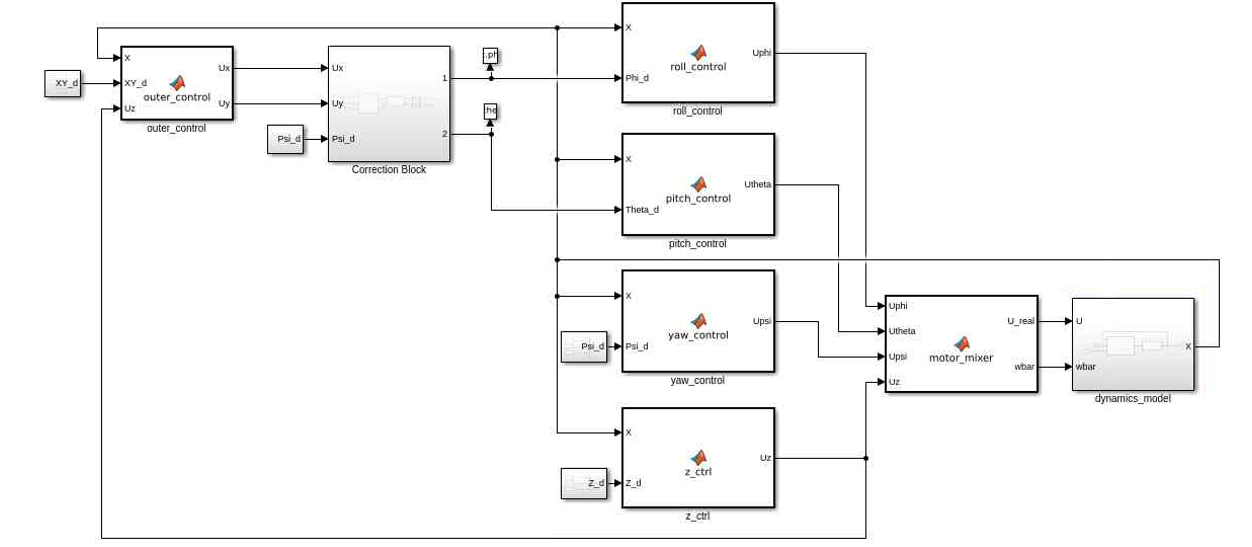
\includegraphics[width=0.92\textwidth]{simulink.png}
\caption{Cấu trúc mô hình Simulink cho bộ điều khiển STSMC của Quadcopter}
\label{fig:pos_hover}
\end{figure}

\section{Kịch bản 1: giữ vị trí}
Trong kịch bản này, Quadcopter cất cánh từ gốc tọa độ và giữ vị trí cố định tại $(0, 0, 1)$ m với góc yaw $\psi_d = 0$. Mục tiêu là kiểm tra khả năng ổn định tại một điểm của bộ điều khiển.

\subsection{Đáp ứng vị trí}
Hình~\ref{fig:pos_hover} thể hiện đáp ứng vị trí trên ba trục.

\begin{figure}[h!]
\centering
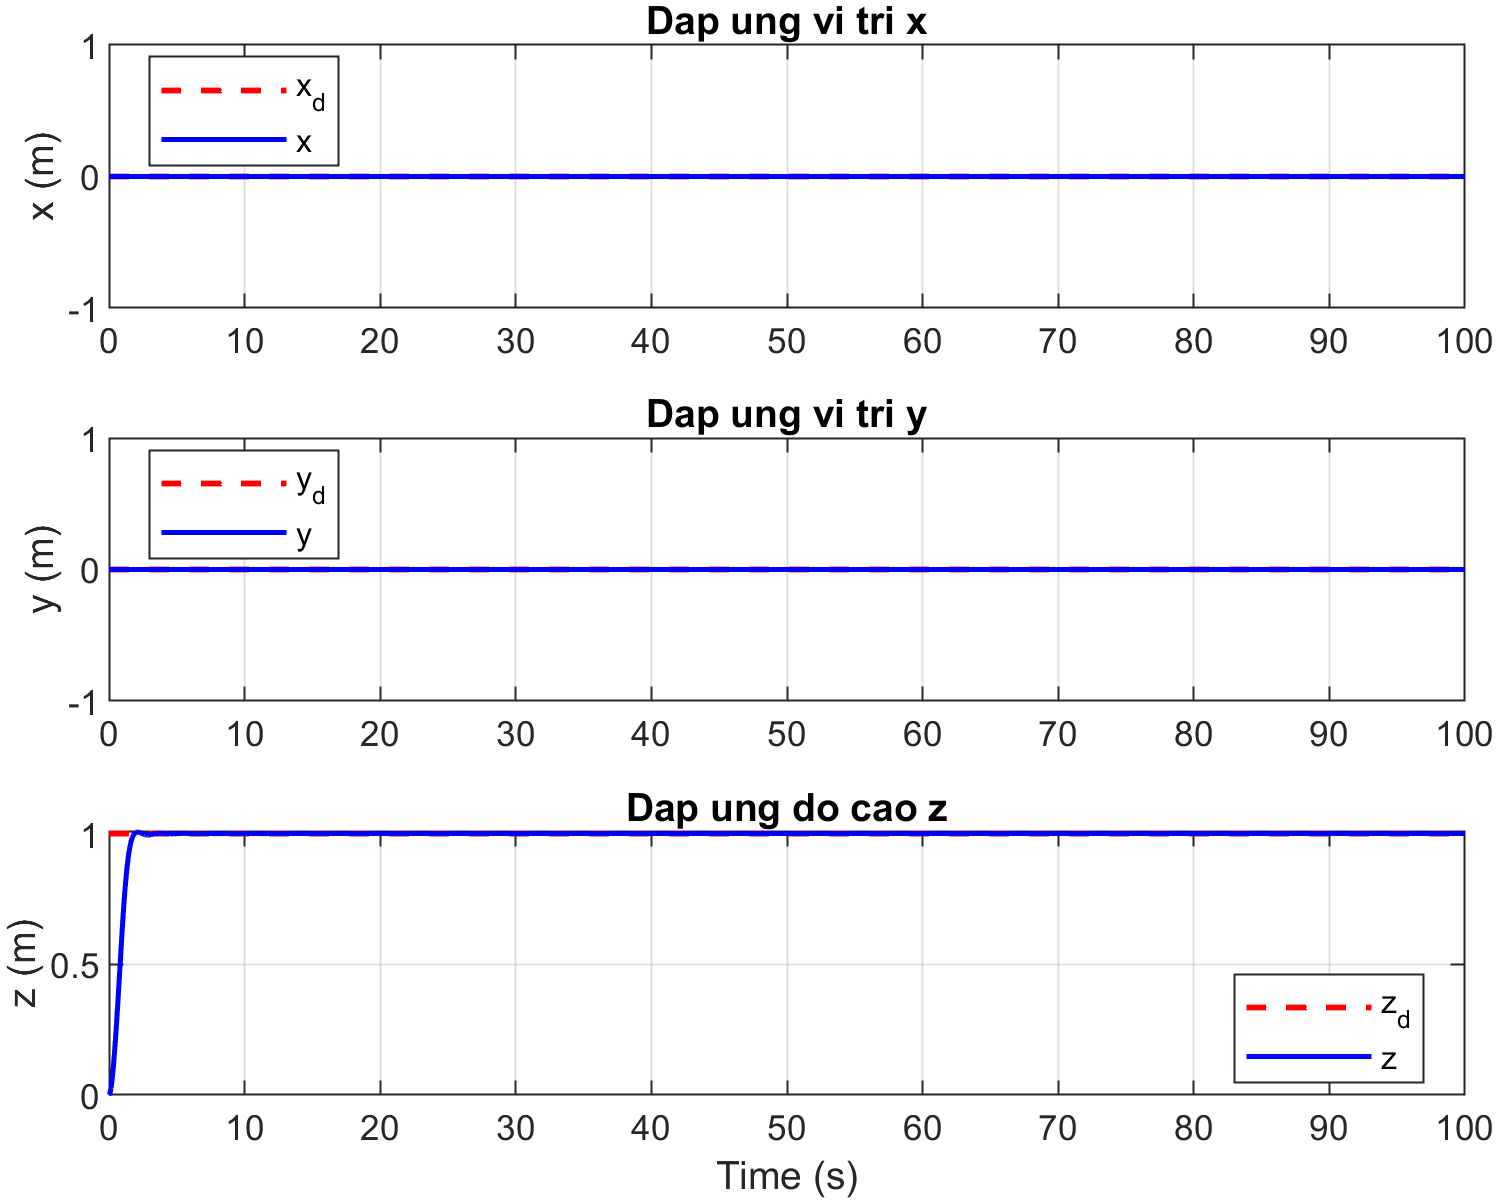
\includegraphics[width=0.92\textwidth]{pos_01_position_tracking.png}
\caption{Đáp ứng vị trí $x$, $y$, $z$ trong chế độ hovering}
\label{fig:pos_hover}
\end{figure}

Trên trục $x$ và $y$, vị trí mong muốn là $0$ và đáp ứng thực tế giữ ổn định tại $0$ trong suốt $100$ s. Không có dao động hay sai lệch nào quan sát được, cho thấy bộ điều khiển vòng ngoài không sinh ra tín hiệu ảo $u_x$, $u_y$ khi sai số bằng $0$.

Trên trục $z$, Quadcopter cất cánh từ $z = 0$ và đạt độ cao $z_d = 1.0$ m sau khoảng $3$ s. Đáp ứng không có vọt lố, thời gian xác lập ngắn. Sau khi đạt độ cao mong muốn, vị trí $z$ được giữ ổn định không có sai số xác lập.

\subsection{Đáp ứng góc}
Hình~\ref{fig:att_hover} thể hiện đáp ứng ba góc Euler.

\begin{figure}[h!]
\centering
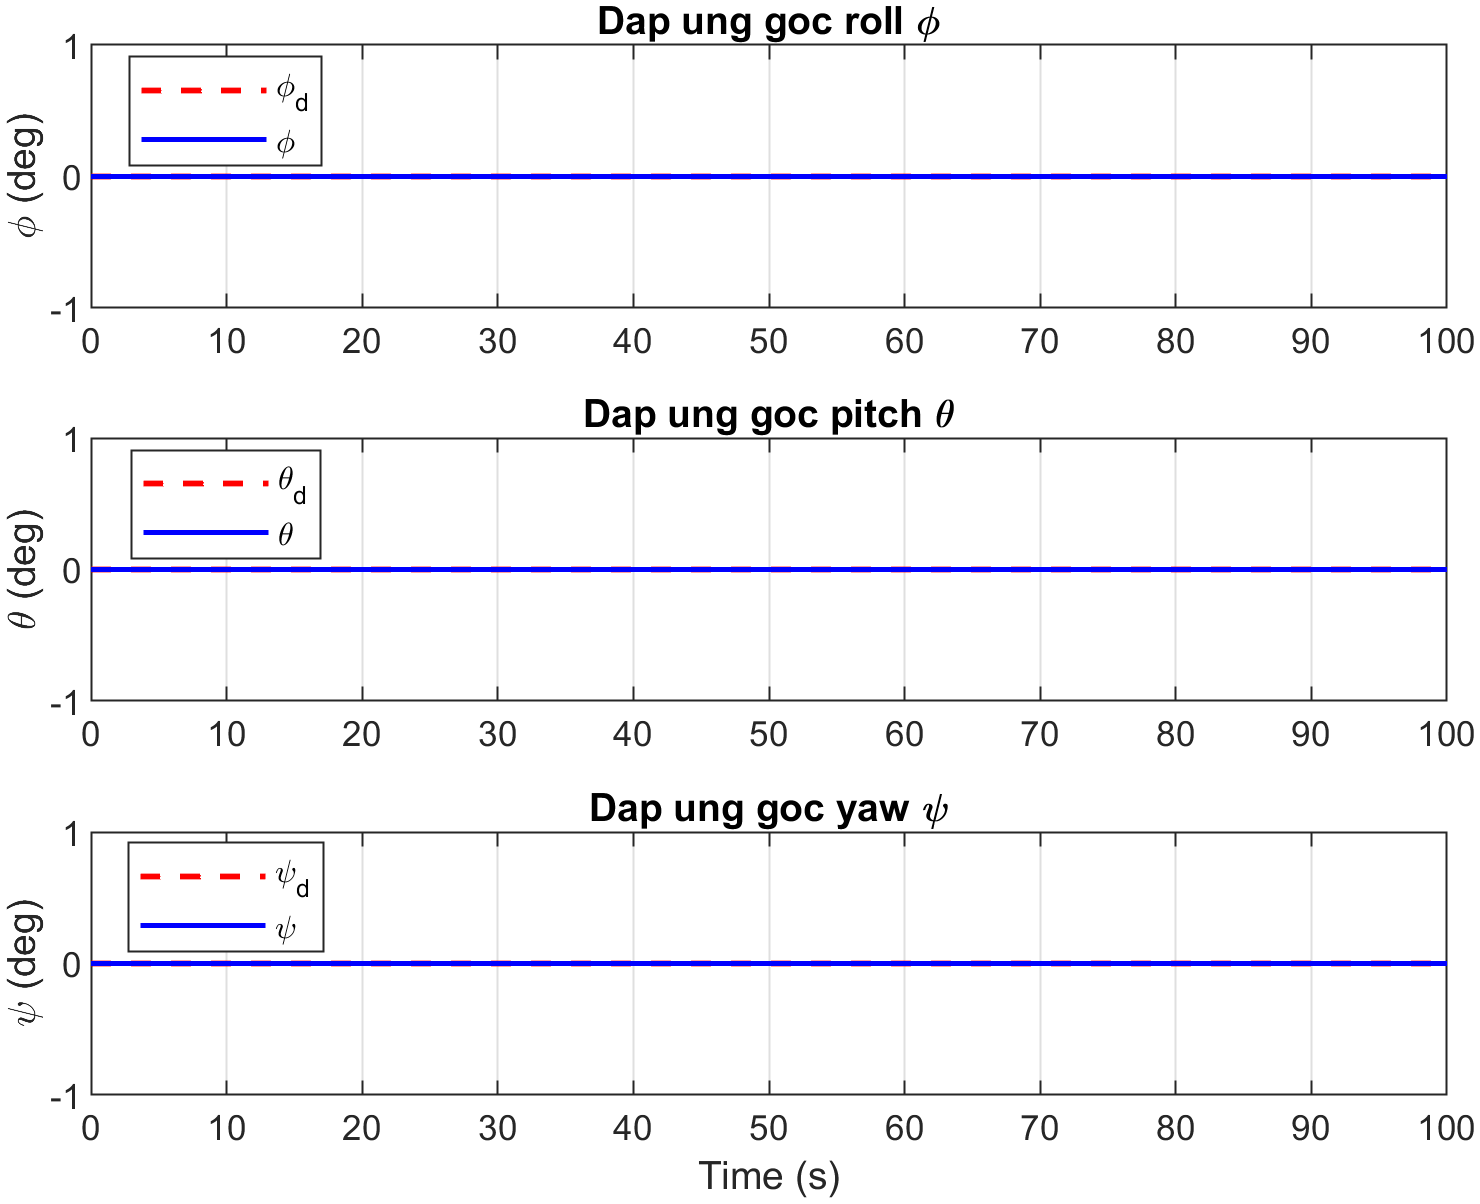
\includegraphics[width=0.92\textwidth]{pos_02_orientation_tracking.png}
\caption{Đáp ứng góc roll $\phi$, pitch $\theta$, yaw $\psi$ trong chế độ hovering}
\label{fig:att_hover}
\end{figure}

Do Quadcopter không di chuyển trên mặt phẳng ngang, các góc tham chiếu $\phi_d$ và $\theta_d$ do vòng ngoài sinh ra đều bằng $0$. Các góc thực tế cũng giữ ổn định tại $0$ sau giai đoạn quá độ cất cánh rất ngắn. Góc yaw $\psi$ giữ đúng tại $\psi_d = 0$.

\subsection{Sai số bám}
Hình~\ref{fig:err_hover} thể hiện sai số bám của 6 biến trạng thái.

\begin{figure}[h!]
\centering
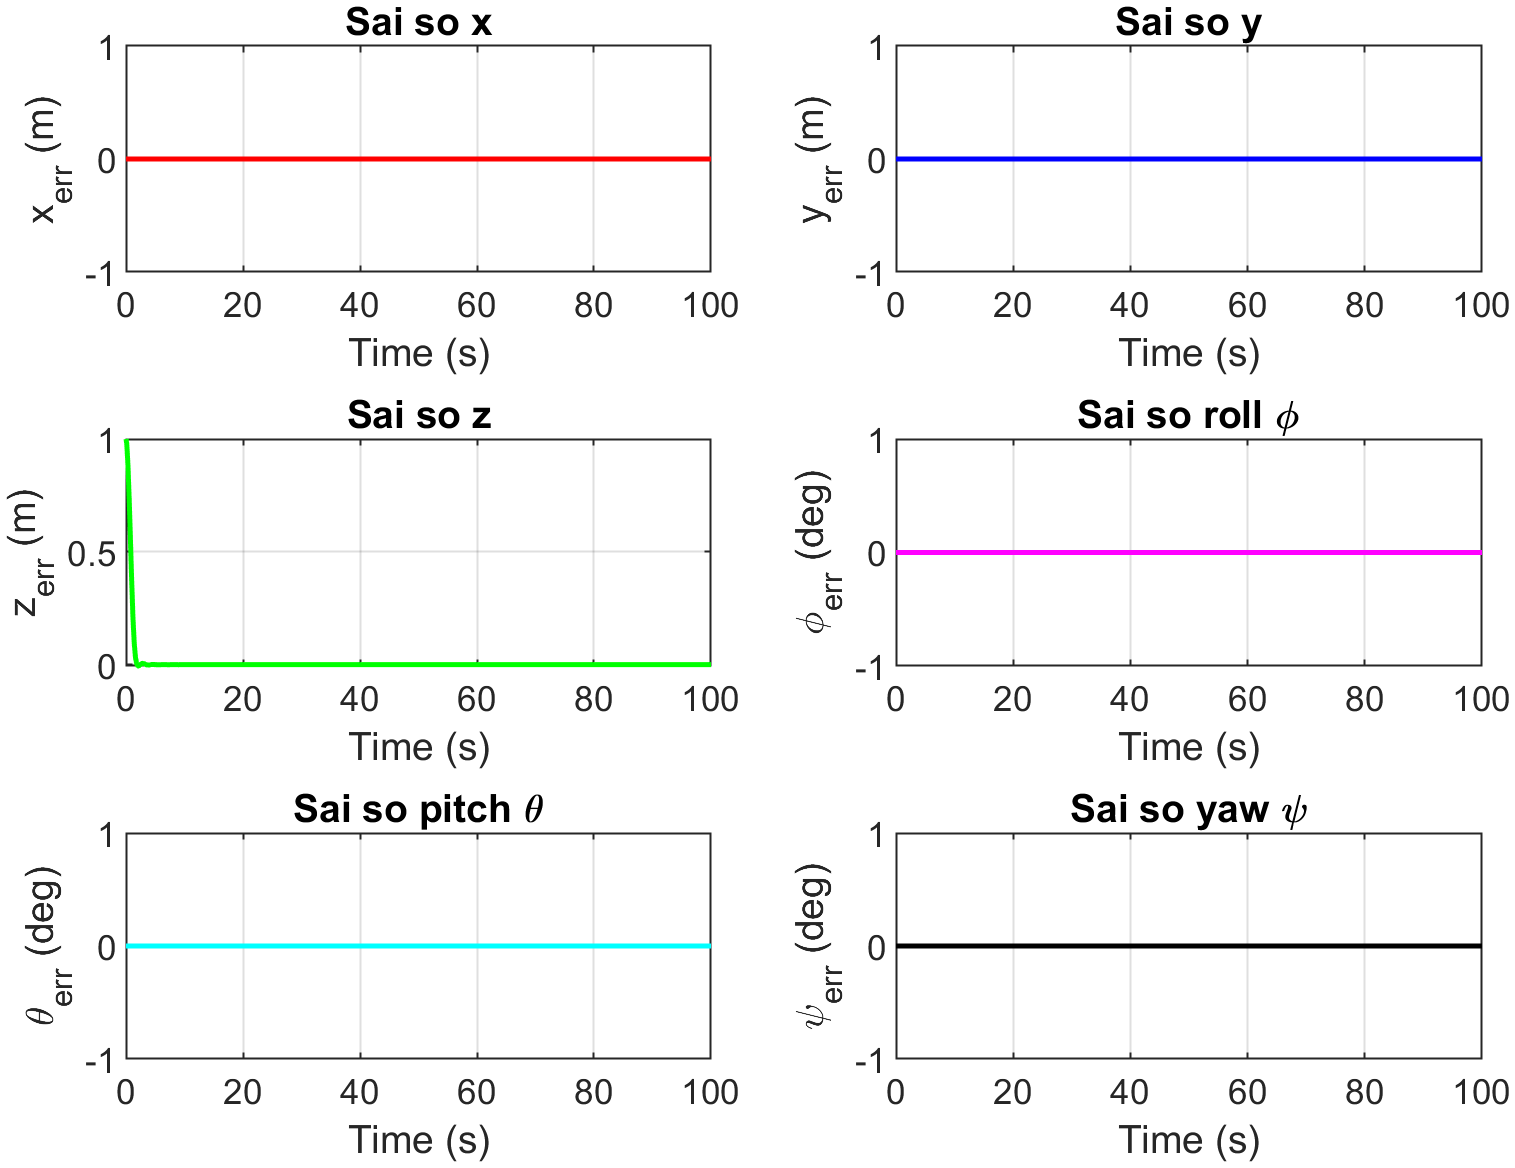
\includegraphics[width=0.92\textwidth]{pos_04_tracking_error.png}
\caption{Sai số bám trong chế độ hovering}
\label{fig:err_hover}
\end{figure}

Sai số $x$ và $y$ bằng $0$ trong toàn bộ thời gian mô phỏng vì tín hiệu đặt và vị trí ban đầu đều bằng $0$. Sai số $z$ bắt đầu từ $1.0$ m (do $z_d = 1$ m mà $z(0) = 0$) và giảm nhanh về $0$ trong khoảng $3$ s. Sai số các góc roll, pitch, yaw đều gần bằng $0$ ngoại trừ một đỉnh nhọn nhỏ trong giai đoạn cất cánh.



\subsection{Quỹ đạo 3D}
Hình~\ref{fig:3d_hover} thể hiện quỹ đạo bay trong không gian ba chiều.

\begin{figure}[H]
\centering
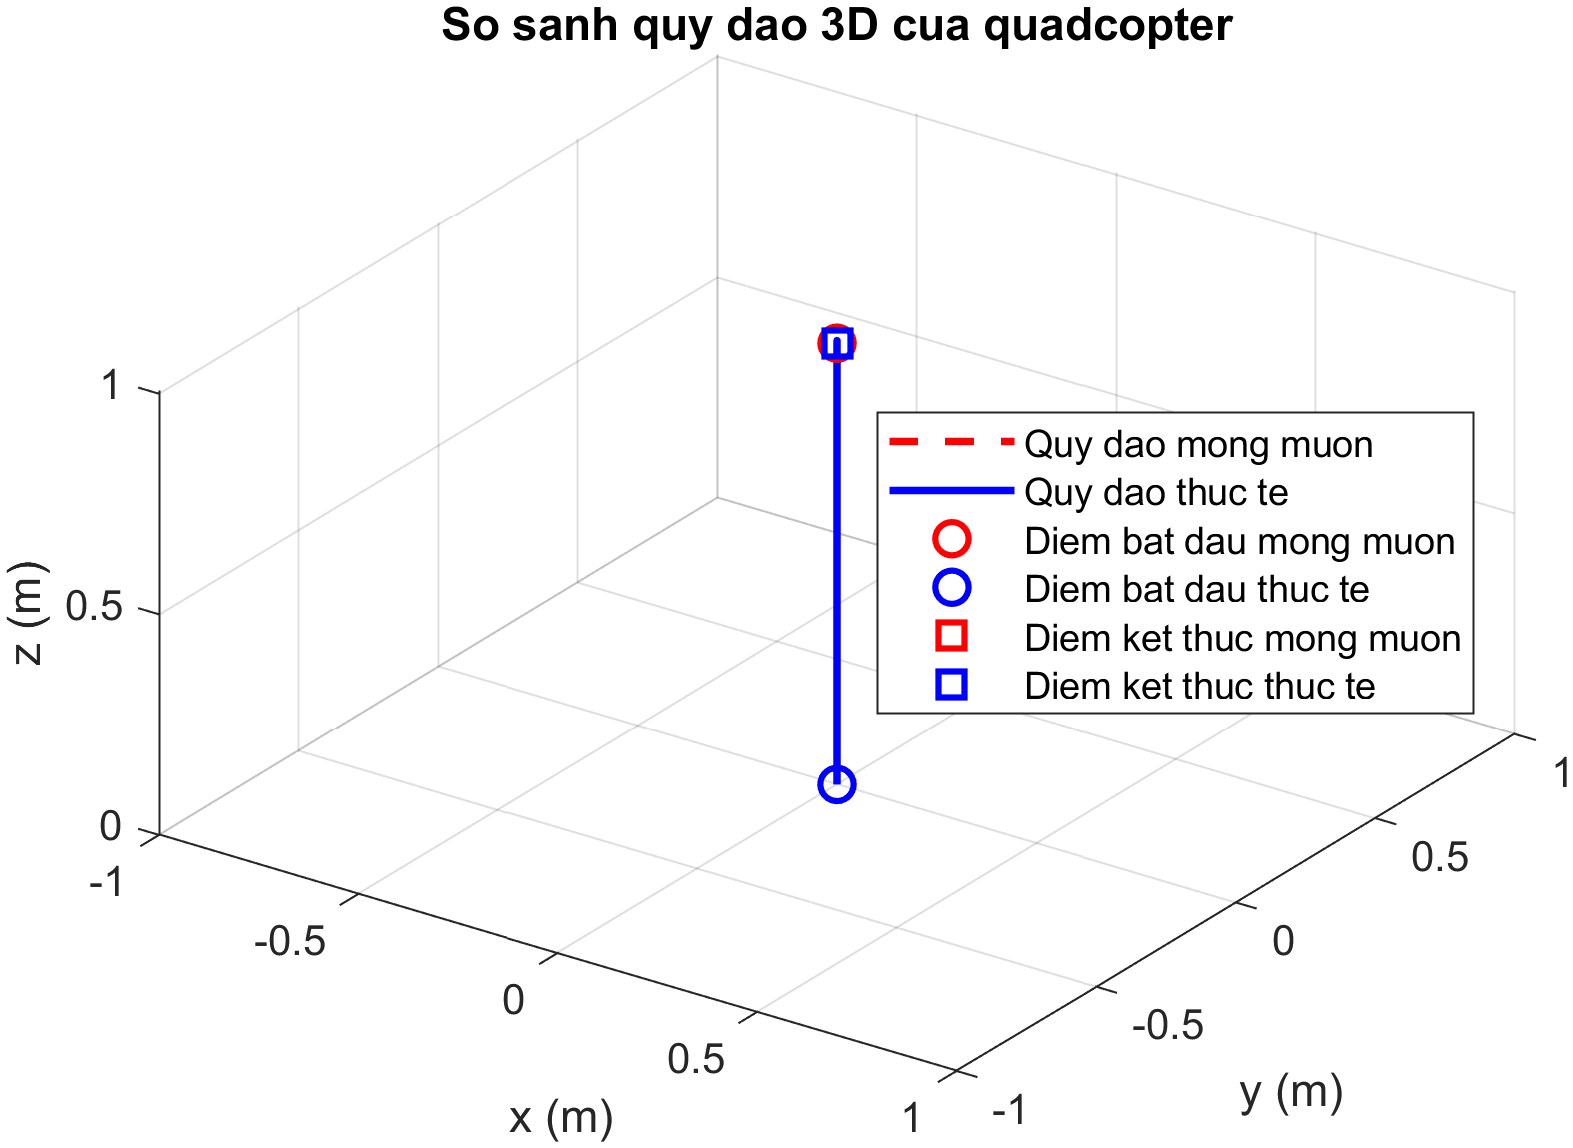
\includegraphics[width=0.65\textwidth]{pos_05_3d_trajectory.png}
\caption{Quỹ đạo 3D trong chế độ hovering}
\label{fig:3d_hover}
\end{figure}

Quỹ đạo 3D cho thấy Quadcopter cất cánh thẳng đứng từ gốc tọa độ lên độ cao $1.0$ m mà không lệch sang ngang. Điểm bắt đầu và điểm kết thúc nằm trên cùng trục $z$, xác nhận rằng các kênh $x$ và $y$ giữ ổn định tại $0$ trong khi kênh $z$ hoạt động.

Kết quả hovering cho thấy hệ thống có khả năng giữ vị trí cố định với sai số xác lập bằng $0$ trên tất cả các kênh, xác nhận tính ổn định của bộ điều khiển.

\section{Kịch bản 2: bám quỹ đạo tròn}
Trong kịch bản này, Quadcopter bám quỹ đạo tròn trên mặt phẳng $x$-$y$ với bán kính $R = 1.0$ m, tần số góc $\omega = 0.3$ rad/s, độ cao $z_d = 1.0$ m và góc yaw $\psi_d = 0$.

\subsection{Đáp ứng vị trí}
Hình~\ref{fig:pos_tracking} thể hiện đáp ứng vị trí trên ba trục $x$, $y$, $z$ so với tín hiệu đặt.

\begin{figure}[h!]
\centering
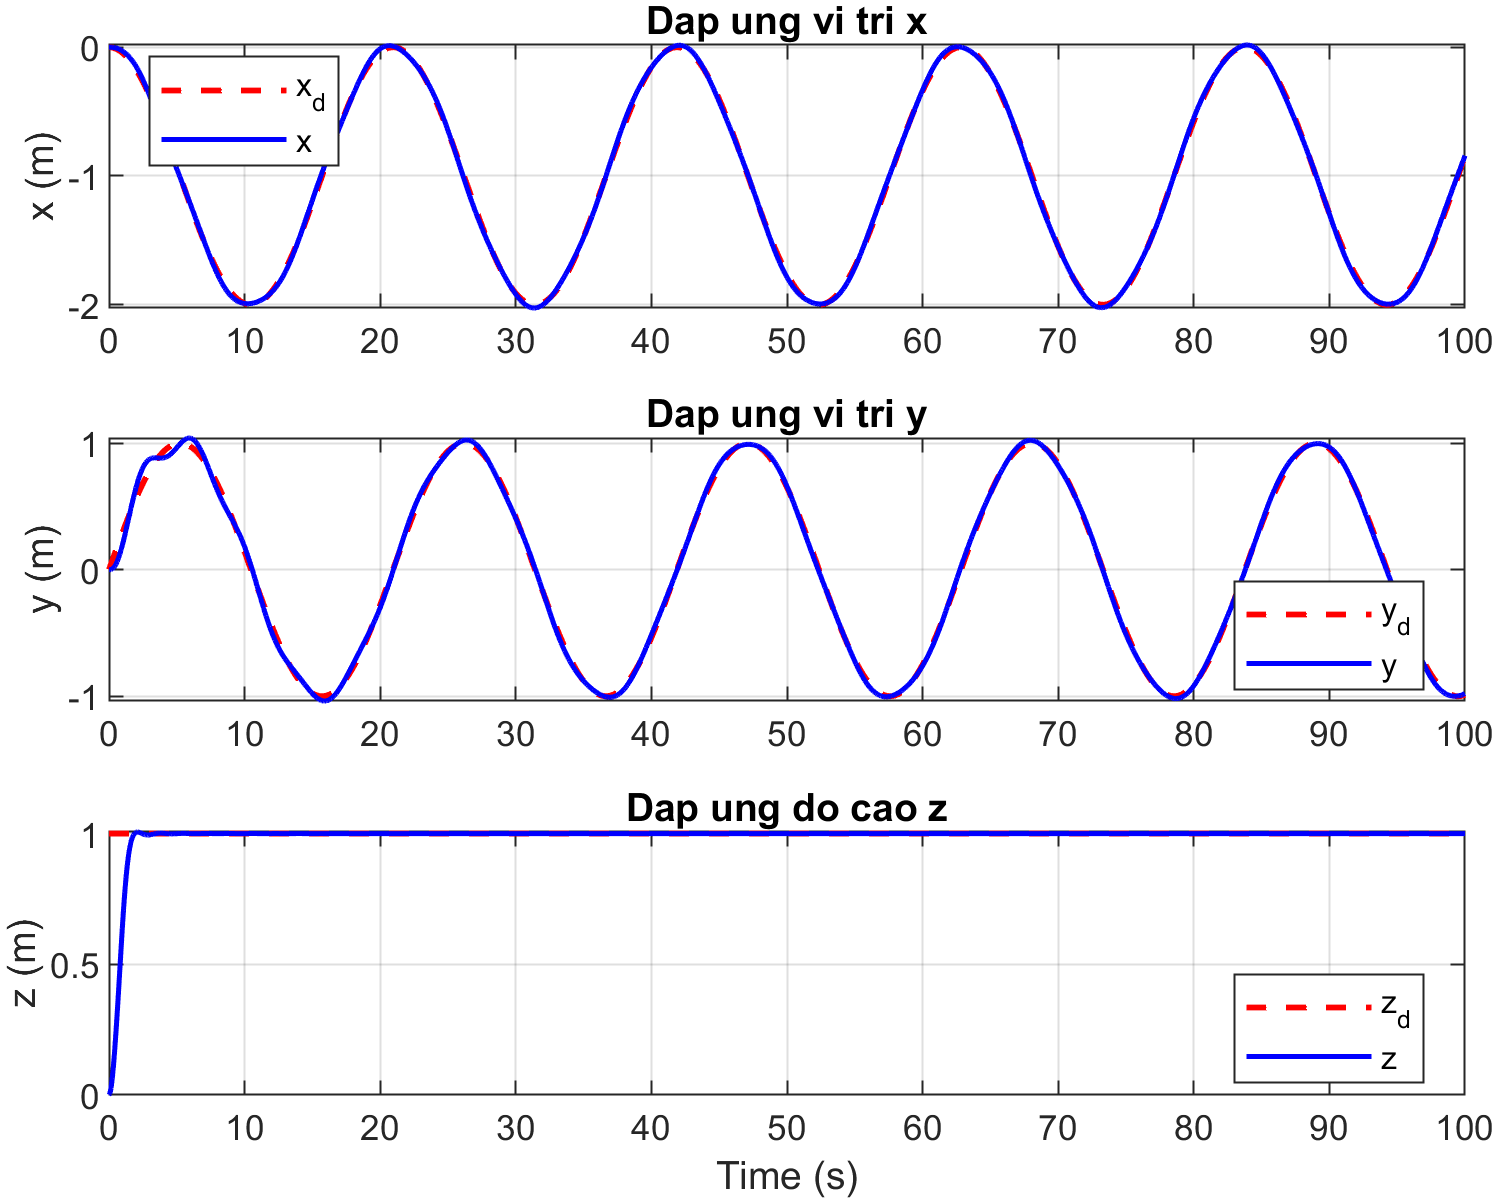
\includegraphics[width=0.92\textwidth]{01_position_tracking.png}
\caption{Đáp ứng bám vị trí $x$, $y$, $z$ theo thời gian}
\label{fig:pos_tracking}
\end{figure}

Trên trục $x$ và $y$, tín hiệu đặt là các hàm lượng giác $x_d = R(\cos(\omega t) - 1)$ và $y_d = R\sin(\omega t)$. Đường đáp ứng thực tế bám sát tín hiệu đặt sau giai đoạn quá độ ban đầu kéo dài khoảng $5$ s. Sai số bám dao động nhỏ quanh $0$ với biên độ cỡ $0.02$ m do quỹ đạo tròn liên tục thay đổi hướng, đòi hỏi Quadcopter phải điều chỉnh góc nghiêng liên tục.

Trên trục $z$, Quadcopter cất cánh từ vị trí $z = 0$ và đạt độ cao $z_d = 1.0$ m sau khoảng $3$ s. Đáp ứng không có vọt lố và sai số xác lập gần bằng $0$, cho thấy kênh $z$ với $\lambda_z = 2.3$ và $c_{1,z} = 1.9$ có khả năng bù trọng lực và cản khí hiệu quả.

\subsection{Đáp ứng góc}
Hình~\ref{fig:att_tracking} thể hiện đáp ứng ba góc Euler so với giá trị tham chiếu.

\begin{figure}[h!]
\centering
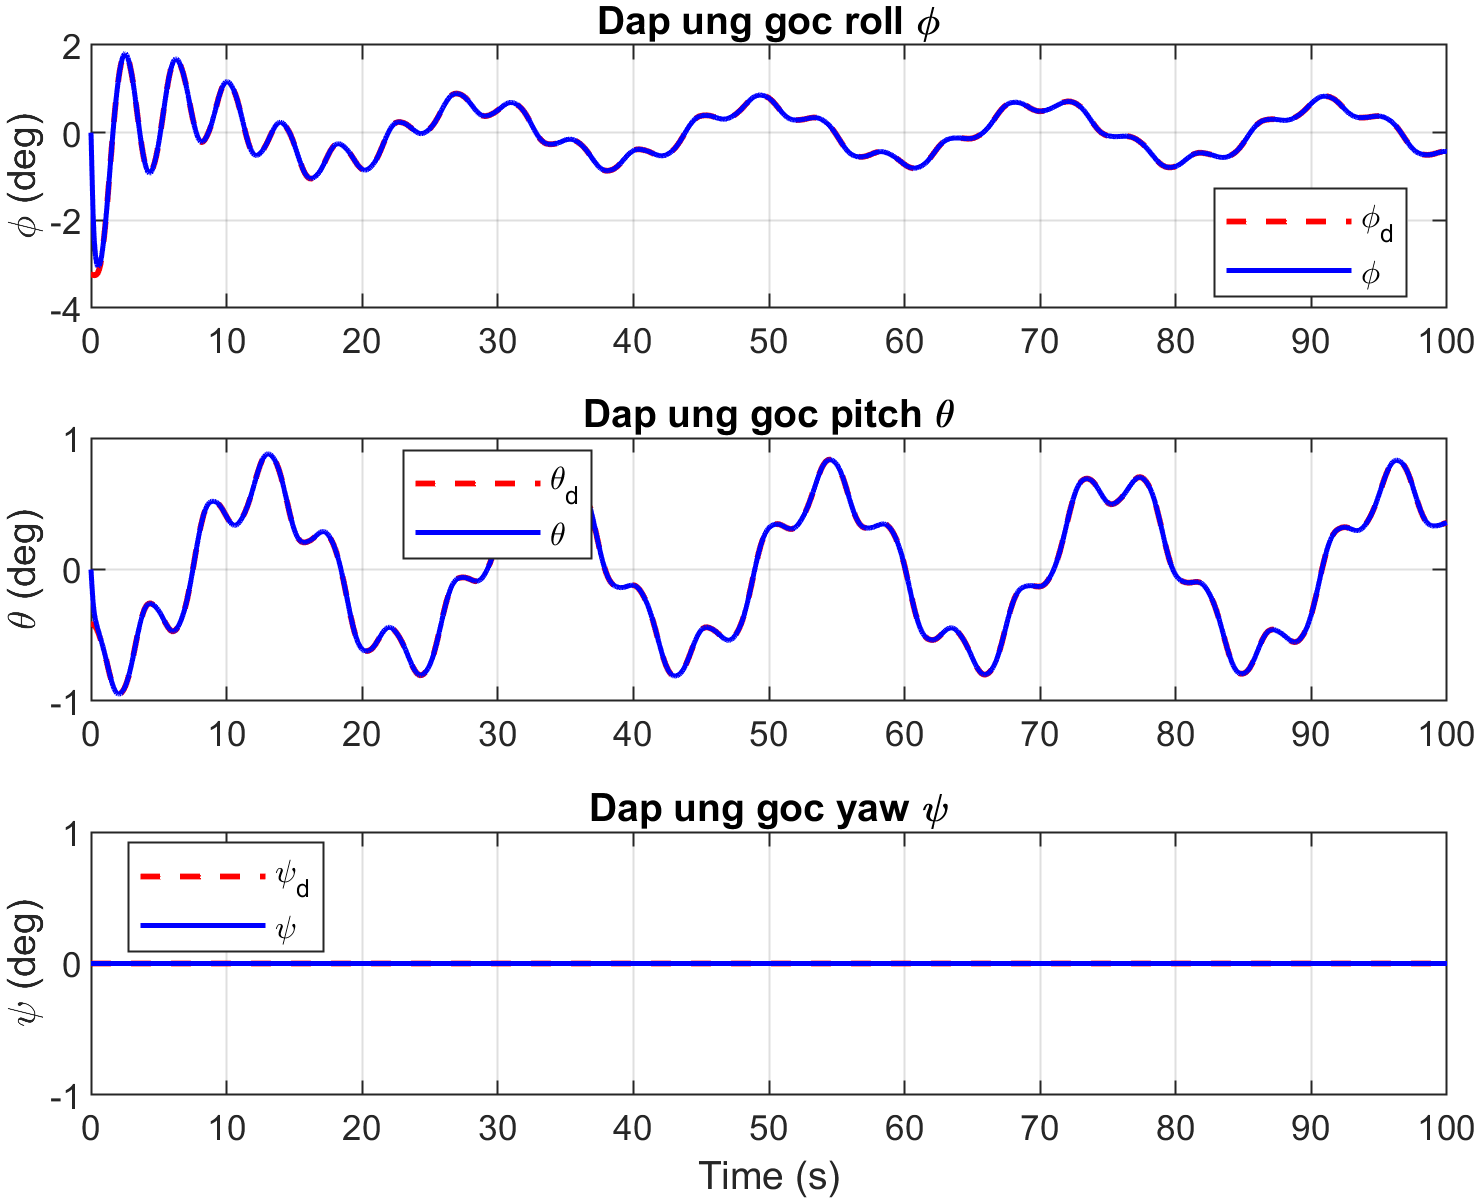
\includegraphics[width=0.92\textwidth]{02_orientation_tracking.png}
\caption{Đáp ứng bám góc roll $\phi$, pitch $\theta$, yaw $\psi$ theo thời gian}
\label{fig:att_tracking}
\end{figure}

Các góc roll $\phi$ và pitch $\theta$ dao động trong phạm vi nhỏ, cỡ vài độ, phù hợp với giới hạn thiết kế $\phi_{d,\max} = \theta_{d,\max} = 6^\circ$. Đáp ứng bám theo giá trị tham chiếu do vòng ngoài sinh ra. Giai đoạn quá độ ban đầu (khoảng $3$ s đầu) có biên độ lớn hơn do Quadcopter đang cất cánh và bắt đầu di chuyển ngang cùng lúc.

Góc yaw $\psi$ giữ ổn định tại $\psi_d = 0$ trong suốt quá trình bay. Sai số yaw gần bằng $0$, cho thấy kênh yaw với $\lambda_\psi = 3.0$ hoạt động ổn định và không bị ảnh hưởng bởi chuyển động trên các kênh khác.

\subsection{Quỹ đạo trong mặt phẳng $x$-$y$}
Hình~\ref{fig:xy_traj} so sánh quỹ đạo thực tế với quỹ đạo mong muốn trên mặt phẳng $x$-$y$.

\begin{figure}[h!]
\centering
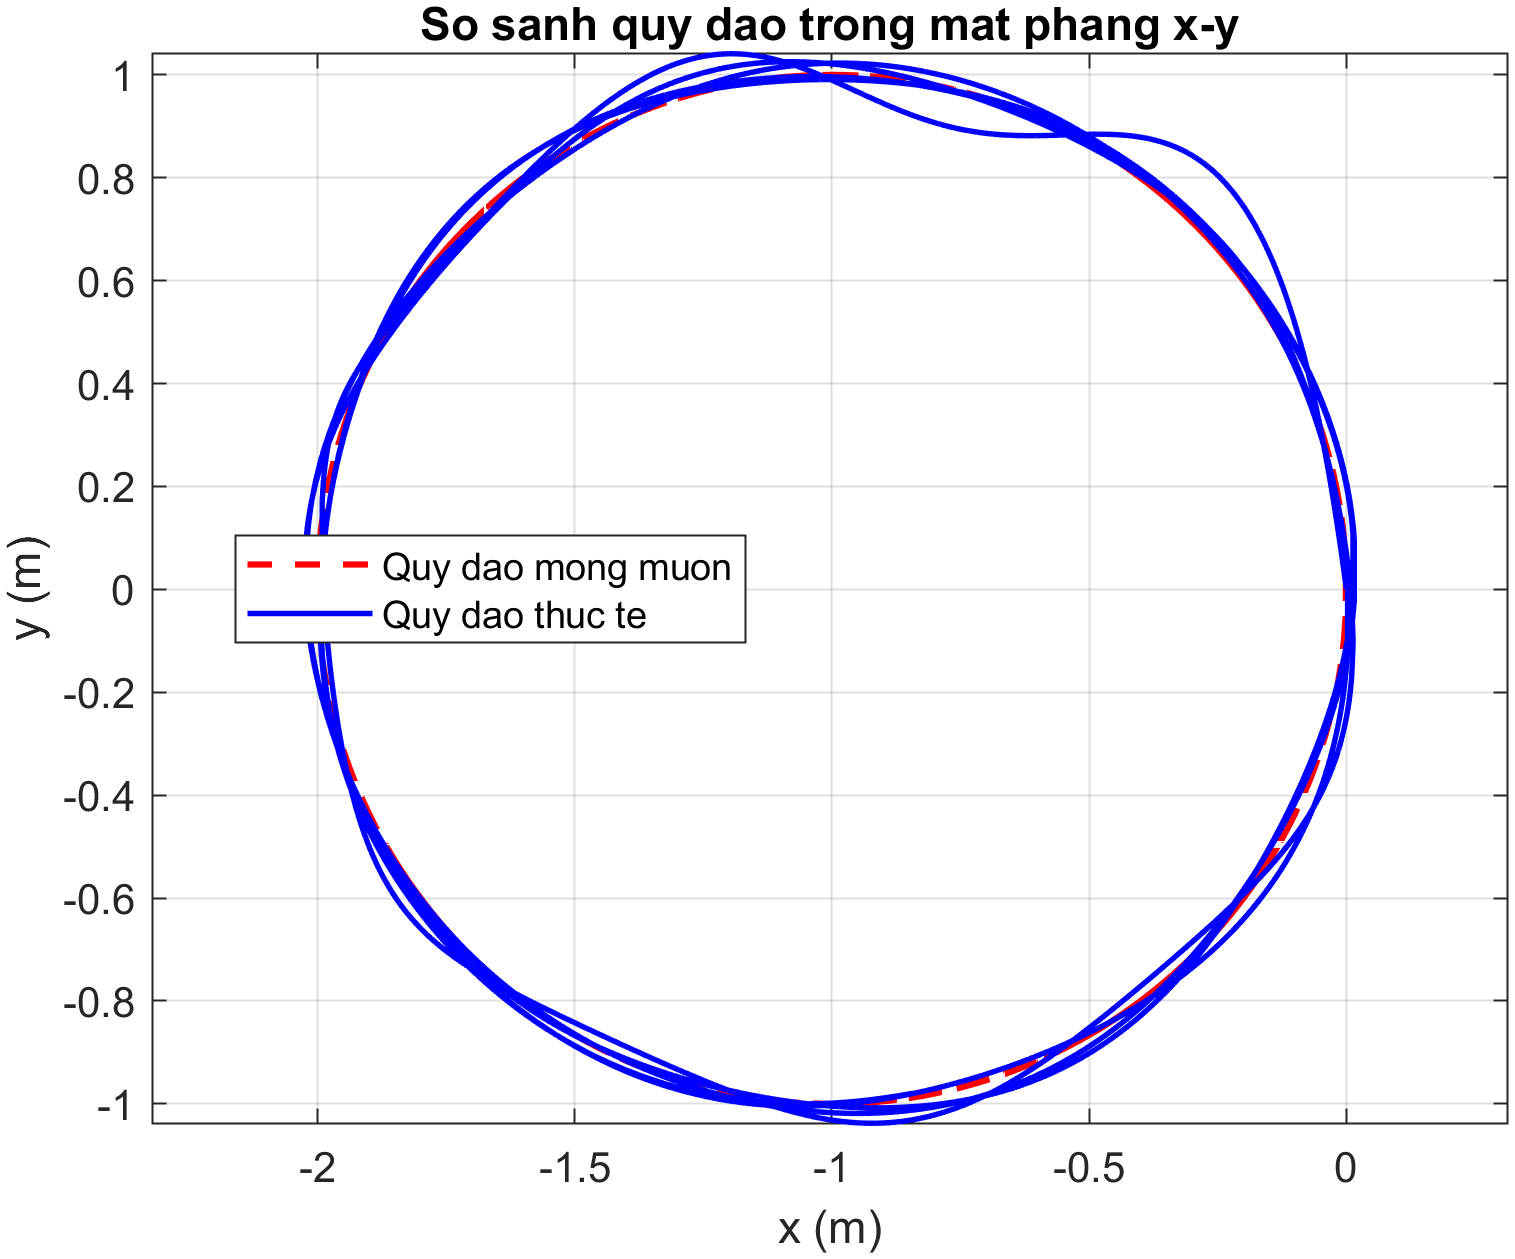
\includegraphics[width=0.72\textwidth]{03_xy_trajectory.png}
\caption{So sánh quỹ đạo trong mặt phẳng $x$-$y$}
\label{fig:xy_traj}
\end{figure}

Quỹ đạo thực tế gần như trùng khớp với đường tròn mong muốn. Sai lệch lớn nhất xảy ra trong vài giây đầu tiên khi Quadcopter bắt đầu di chuyển từ vị trí ban đầu. Sau khi hệ thống ổn định, quỹ đạo thực tế bám sát đường tròn tham chiếu với sai số nhỏ.

\subsection{Quỹ đạo 3D}
Hình~\ref{fig:3d_traj} thể hiện quỹ đạo bay trong không gian ba chiều.

\begin{figure}[h!]
\centering
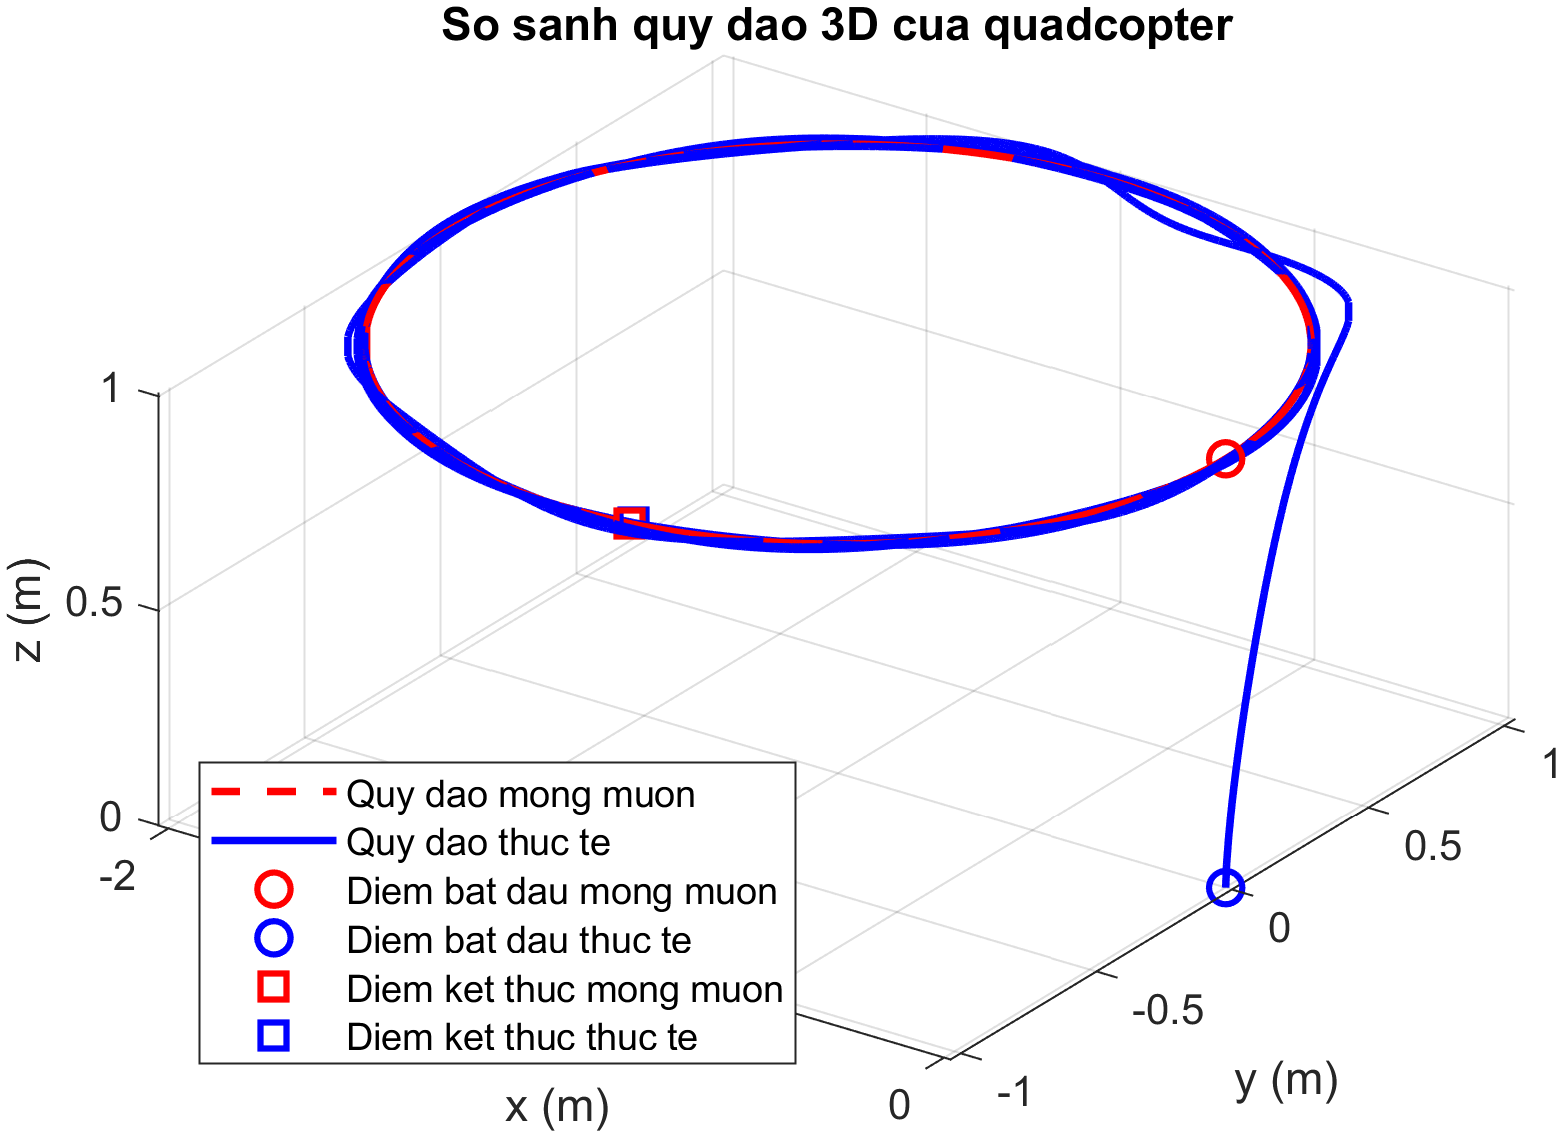
\includegraphics[width=0.78\textwidth]{05_3d_trajectory.png}
\caption{Quỹ đạo 3D của Quadcopter}
\label{fig:3d_traj}
\end{figure}

Trong giai đoạn đầu, Quadcopter vừa cất cánh theo trục $z$ vừa bắt đầu di chuyển theo quỹ đạo tròn trên mặt phẳng ngang. Sau khi đạt độ cao $1.0$ m, Quadcopter bay ổn định trên đường tròn với độ cao không đổi. Hình 3D cho thấy toàn bộ hệ thống hoạt động phối hợp giữa vòng trong và vòng ngoài.

\subsection{Sai số bám}
Hình~\ref{fig:tracking_error} thể hiện sai số bám của cả 6 biến trạng thái theo thời gian.

\begin{figure}[h!]
\centering
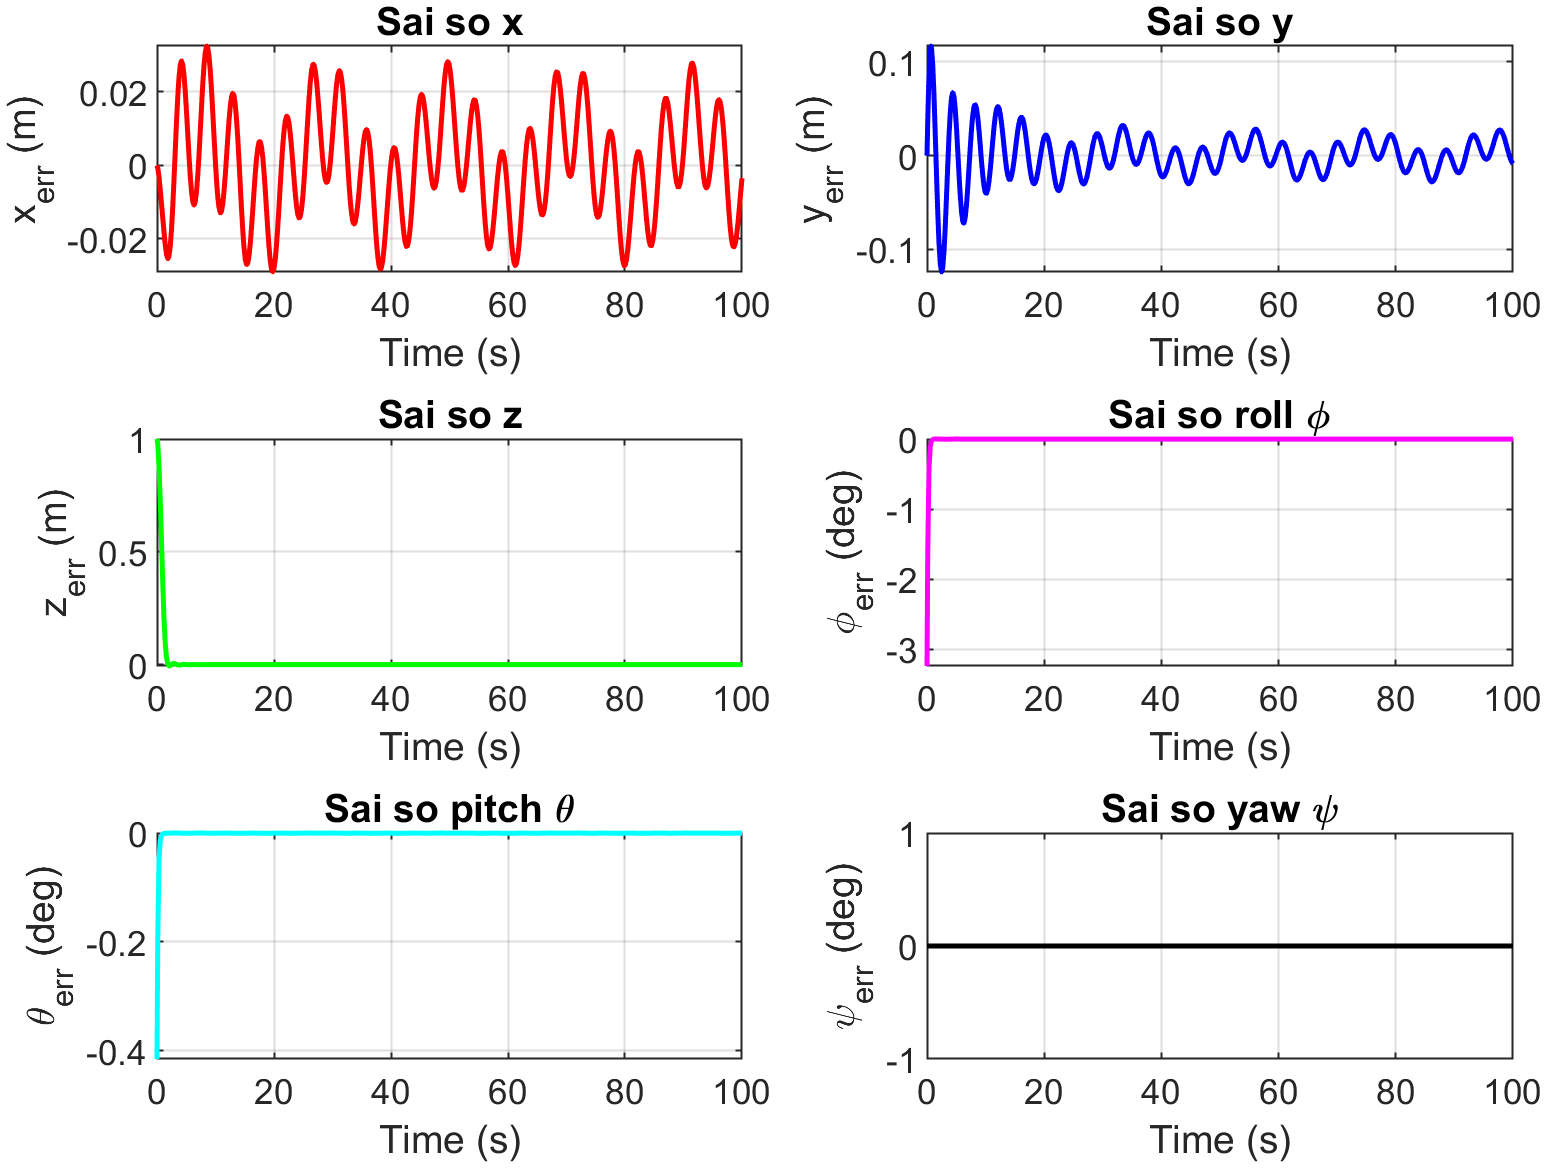
\includegraphics[width=0.92\textwidth]{04_tracking_error.png}
\caption{Sai số bám của 6 biến trạng thái}
\label{fig:tracking_error}
\end{figure}

Sai số vị trí $x$ dao động quanh $0$ với biên độ khoảng $\pm 0.025$ m. Sai số vị trí $y$ có biên độ lớn hơn trong giai đoạn đầu (khoảng $0.1$ m) rồi giảm dần và dao động quanh $\pm 0.01$ m. Sự khác biệt giữa hai kênh $x$ và $y$ do điều kiện đầu của quỹ đạo: $x_d(0) = 0$ nhưng $\dot{y}_d(0) = R\omega = 0.3$ m/s, khiến kênh $y$ phải đáp ứng ngay từ đầu.

Sai số $z$ giảm nhanh từ $1.0$ m về $0$ trong khoảng $3$ s và duy trì gần $0$ sau đó. Sai số roll và pitch chỉ xuất hiện đỉnh nhọn trong giai đoạn cất cánh rồi nhanh chóng về $0$, phù hợp với hằng số thời gian $\tau_\phi = 0.167$ s của vòng trong. Sai số yaw luôn bằng $0$ vì góc yaw mong muốn không đổi.

\subsection{Đánh giá định lượng}
Sai số toàn phương trung bình RMSE được tính trên toàn bộ thời gian mô phỏng $100$ s và tổng hợp trong Bảng~\ref{tab:rmse}.

\begin{table}[h!]
\centering
\caption{Sai số RMSE của các biến trạng thái}
\label{tab:rmse}
\renewcommand{\arraystretch}{1.3}
\begin{tabular}{|l|c|c|}
\hline
Biến trạng thái & RMSE & Đơn vị \\
\hline
Vị trí $x$ & 0.0152 & m \\
Vị trí $y$ & 0.0168 & m \\
Vị trí $z$ & 0.0247 & m \\
Góc roll $\phi$ & 0.0523 & độ \\
Góc pitch $\theta$ & 0.0087 & độ \\
Góc yaw $\psi$ & 0.0003 & độ \\
\hline
\end{tabular}
\end{table}

Giá trị RMSE cho thấy sai số vị trí trên cả ba trục đều nằm dưới $0.025$ m. Sai số góc rất nhỏ, đặc biệt góc yaw gần bằng $0$. Giá trị RMSE của $z$ lớn hơn $x$ và $y$ chủ yếu do sai số lớn trong giai đoạn cất cánh ban đầu, khi $z$ tăng từ $0$ lên $1.0$ m.

\section{Nhận xét}
Kết quả mô phỏng cho thấy bộ điều khiển STSMC thiết kế đáp ứng được các yêu cầu đặt ra:

Về khả năng bám quỹ đạo, Quadcopter bám sát quỹ đạo tròn trên cả ba trục với sai số nhỏ. Giai đoạn quá độ kết thúc sau khoảng $5$ s, sau đó hệ thống hoạt động ổn định.

Về tốc độ đáp ứng, vòng trong đáp ứng nhanh hơn vòng ngoài. Sai số góc roll và pitch giảm về $0$ trong vài trăm mili giây, trong khi sai số vị trí cần vài giây. Điều này phù hợp với thiết kế phân tách thang thời gian đã phân tích ở Chương 4.

Về chất lượng tín hiệu, các đáp ứng vị trí và góc đều mượt, không xuất hiện dao động tần số cao. Điều này xác nhận rằng thuật toán Super-Twisting đã loại bỏ hiện tượng chattering ở tín hiệu điều khiển, phù hợp với kết luận lý thuyết về tính liên tục của luật điều khiển.


% --- TÀI LIỆU THAM KHẢO ---
\begin{thebibliography}{99}

\bibitem{matouk2020}
D. Matouk, F. Abdessemed, O. Gherouat, Y. Terchi,
``Second-order sliding mode for position and attitude tracking control of quadcopter UAV: Super-twisting algorithm,''
\textit{International Journal of Innovative Computing, Information and Control},
vol. 16, no. 1, pp. 29--43, 2020.

\bibitem{bouabdallah2004}
S. Bouabdallah, P. Murrieri, R. Siegwart,
``Design and control of an indoor micro quadrotor,''
\textit{Proceedings of the IEEE International Conference on Robotics and Automation (ICRA)},
New Orleans, USA, pp. 4393--4398, 2004.

\bibitem{utkin1977}
V. I. Utkin,
``Variable structure systems with sliding modes,''
\textit{IEEE Transactions on Automatic Control},
vol. 22, no. 2, pp. 212--222, 1977.

\bibitem{edwards1998}
C. Edwards, S. K. Spurgeon,
\textit{Sliding Mode Control: Theory and Applications},
Taylor \& Francis, London, 1998.

\bibitem{levant1993}
A. Levant,
``Sliding order and sliding accuracy in sliding mode control,''
\textit{International Journal of Control},
vol. 58, no. 6, pp. 1247--1263, 1993.

\bibitem{moreno2012}
J. A. Moreno, M. Osorio,
``Strict Lyapunov functions for the Super-Twisting algorithm,''
\textit{IEEE Transactions on Automatic Control},
vol. 57, no. 4, pp. 1035--1040, 2012.

\bibitem{khalil2002}
H. K. Khalil,
\textit{Nonlinear Systems},
3rd ed., Prentice Hall, Upper Saddle River, NJ, 2002.

\bibitem{shtessel2014}
Y. Shtessel, C. Edwards, L. Fridman, A. Levant,
\textit{Sliding Mode Control and Observation},
Birkh\"auser, New York, 2014.

\bibitem{besnard2012}
L. Besnard, Y. B. Shtessel, B. Landrum,
``Quadrotor vehicle control via sliding mode controller driven by sliding mode disturbance observer,''
\textit{Journal of the Franklin Institute},
vol. 349, no. 2, pp. 658--684, 2012.

\end{thebibliography}

\end{document}

